\chapter{Digital Video Stabilization using IMUs} \label{chapter_four}

In the past chapters, the challenges associated and methods available were discussed. This chapter contains the process we used to digitally stabilize video for our use-case. This chapter now proposed methods to digitally stabilize videos with large focal lengths using inertial data for pose estimation alone. Figure \ref{fig:dis_pipeline} depicts a general flowchart of the the developed pipeline.

% \begin{sidewaysfigure}
%     \centering
%     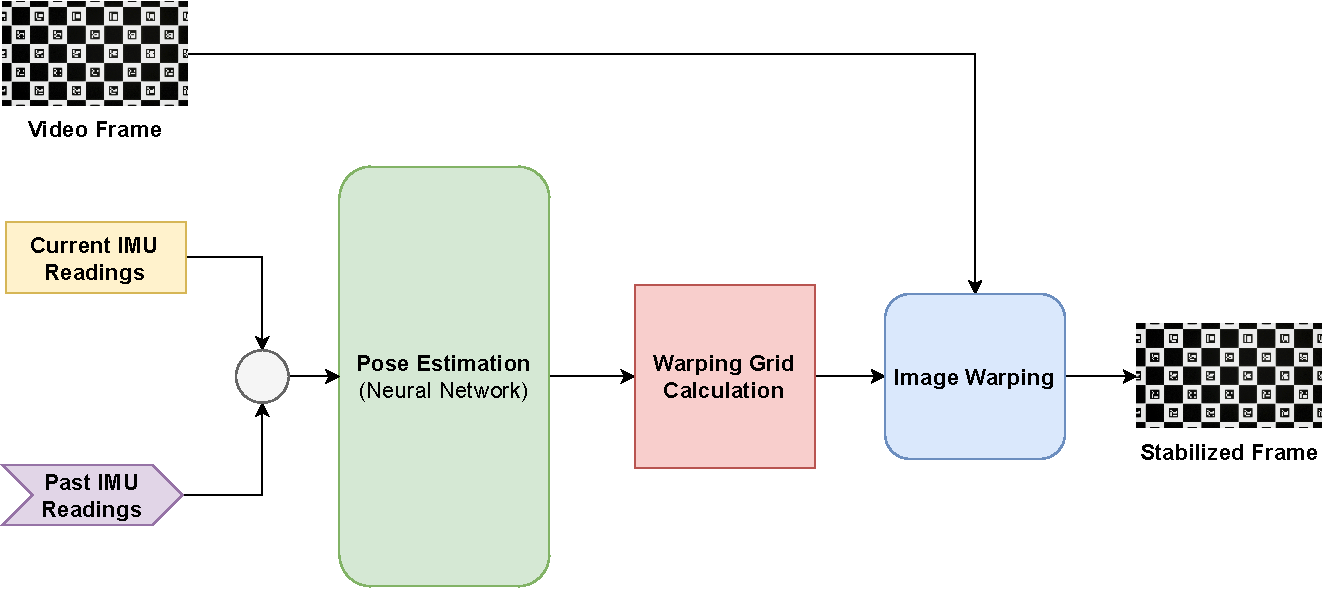
\includegraphics[scale=0.9]{images/fig_chapter4/dis_pipleline.pdf}
%     \caption{DIS pipeline using IMU Sensor}
%     \label{fig:dis_pipeline}
% \end{sidewaysfigure}

\begin{figure}[H]
    % \centering
    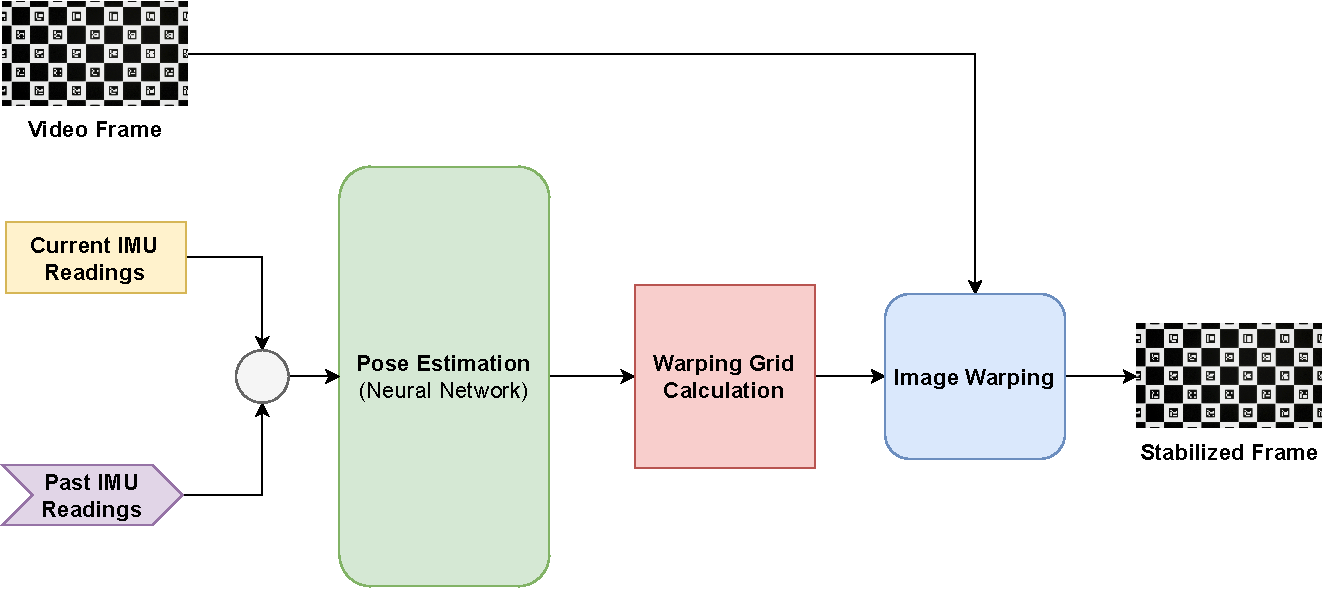
\includegraphics[scale=0.58]{images/fig_chapter4/dis_pipleline.pdf}
    \caption{Flowchart of a DVS pipeline using a IMU for pose estimation}
    \label{fig:dis_pipeline}
\end{figure}

In this work, an IMU sensor will be used for camera pose estimation that is a prerequisite for video stabilization. Based on the accuracy requirements for the camera pose estimation algorithm a data-driven neural network approach will be used, as classical signal processing combined with filtering failed to provide the required accuracy over longer periods of time due to severe drift. To be able to train the models to the required accuracy, a combination of simulated and real data is used. To capture the video we are using a GoPro Hero 10 which provides synchronised image and sensor data capture. The factory wide FoV lens was swapped to a low field of view lens having a large focal length (depicted in figure \ref{fig:mod_gopro_hero10}). The simulation was build using Unreal Engine 4 and Microsoft AirSim. Table \ref{tab:technical_details} shows the technical specifications of the camera setup. For simulation similar camera parameters were used.

\begin{table}[H]
    \centering
\begin{tabular}{ c| c | L }

     Image Sensor & 
     Sony & 
     Diagonal 7.85 mm (Type 1/2.3) 23.91 M CMOS Image Sensor with Square Pixel. \\
     \hline
     
     IMU Sensor & 
     Bosch & 
     6-axis IMU Sensor
     Accelerometer (A): 16-bit or 0.06 mg/LSB 
     Gyroscope (G): 16-bit or 0.004 dps/LSB  \\
     \hline
     
     Lens & 
     Zeiss & 
     15° FOV and 200 mm focal length \\

\end{tabular}
    \caption{Hardware technical specifications}
    \label{tab:technical_details}
\end{table}

\begin{figure}[H]
    \centering
    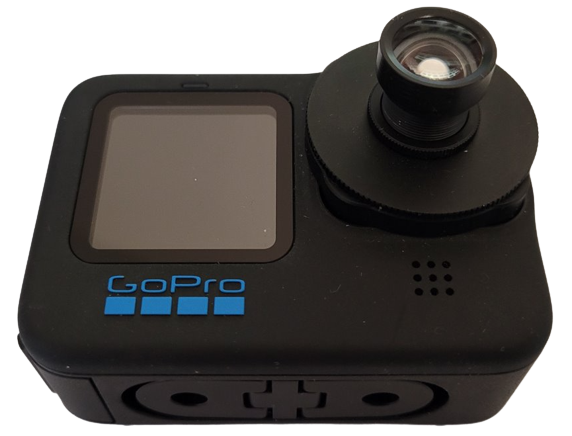
\includegraphics[scale=0.25]{images/fig_chapter4/mod_gorpro_hero_10.png}
    \caption{Modified GoPro Hero 10 with large focal length lens}
    \label{fig:mod_gopro_hero10}
\end{figure}

\begin{figure}[H]
    \centering
    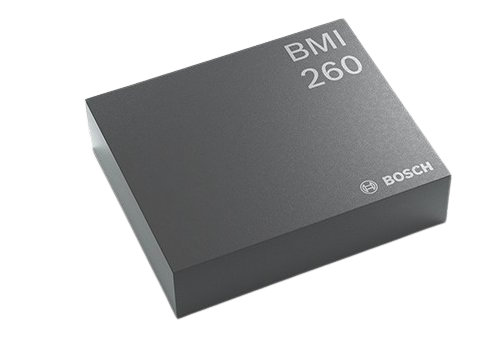
\includegraphics[scale=0.2]{images/fig_chapter4/bmi260.png}
    \caption{Bosch BMI260 IMU Sensor}
    \label{fig:imu_bmi260}
\end{figure}

\section{Data Collection}
Collecting enough data for any data driven learning approach is cumbersome and sometimes an iterative process. The data or training data in this case are the readings coming from the IMU sensor and the target (ground truth) being the camera pose (position and orientation). Real data was collected by mounting the camera on a rig which had vibrations associated with it on movement (figure \ref{fig:camera_rig}). We made sure that the data depicts real life scenarios by moving the rig around in many different ways and let it vibrate and collect the data. The ground truth camera and IMU poses as well as all calibration parameters like camera intrinsics, IMU parameters and transformations between the sensor coordinate frames were generated using proprietary Zeiss software and is beyond the scope of this work.

\begin{figure}[H]
    \centering
    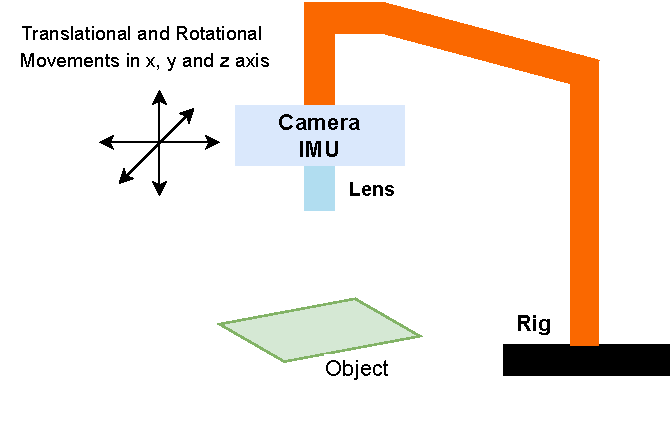
\includegraphics[scale=0.8]{images/fig_chapter4/camera_rig.pdf}
    \caption{Camera setup}
    \label{fig:camera_rig}
\end{figure}

As generating enough real data is time consuming, the motion patterns were analyzed and a simulation was created to generate more training data. Generating simulated data with accurate ground truth is a fast processes not requiring much post-processing. This also allowed us to vary the noise characteristics of the simulated IMU data to make the neural network robust and generalize well.

\subsection{Data Analysis}
\label{sec:data_analysis}
The data recorded from the real world camera setup was analysed to determine the vibration and IMU noise characteristics. Table \ref{tab:imu_noise_characteristics} summarises the white noise and bias characteristics determined from the raw IMU Sensor Readings. 

% These match closely with the data provided by the manufacturer. Accelerometer variance from data sheet $ 160 \mu g /\sqrt{Hz} $ and for gyroscope $ 0.008 dps /\sqrt{Hz}  $.

\begin{table}[H]
\centering
\begin{tabular}{l|c}
    \textbf{Parameter} & \textbf{Value} \\ \hline
    Accelerometer White Noise & $ \mu = 0 $ and $ \sigma^{2}=0.3$x$10^{-3} m/s^{2}$  \\  
    Gyro White Noise & $ \mu = 0 $ and $ \sigma^{2}=2.8$x$10^{-6} rad/s$ \\  
\end{tabular}
\caption{IMU noise characteristics}
\label{tab:imu_noise_characteristics}
\end{table}


% \begin{table}[H]
% \centering
% \begin{tabular}{l|c}
%     \textbf{Parameter} & \textbf{Value} \\ \hline
%     Accelerometer Bias & xx \\  
%     Accelerometer White Noise & $ \mu = 0 $ and $ \sigma^{2}=0.00038 m/s^{2}$ \\  
%     Gyro Bias & xx \\  
%     Gyro White Noise & $ \mu = 0 $ and $ \sigma^{2}=0.xxx $ \\  
% \end{tabular}
% \caption{IMU Noise Characteristics}
% \label{tab:imu_noise_characteristics}
% \end{table}

Apart from the IMU noise characteristics the vibrations from the real ground truth data were analyzed. These vibration characteristics are important to understand their and to set the Simulation parameters. Vibrations are characterised by \textbf{Amplitude} ( A or  $ \theta $), \textbf{Time Constant} $ \tau $ and \textbf{Frequency} $ \omega $. We have damped oscillations for both translational and rotational vibrations as shown in figure \ref{fig:damped_vib} and can be characterised by the equations \ref{eqn:vib_disp} and \ref{eqn:vib_rot}.

\begin{equation}
  \label{eqn:vib_disp}
  \begin{aligned}
    A(t) = Ae^{-t/\tau}sin(2\pi\omega t) \\
  \end{aligned}
\end{equation}

\begin{equation}
  \label{eqn:vib_rot}
  \begin{aligned}
    \theta(t) = \theta e^{-t/\tau}sin(2\pi\omega t) \\
  \end{aligned}
\end{equation}

\begin{figure}[H]
    \centering
    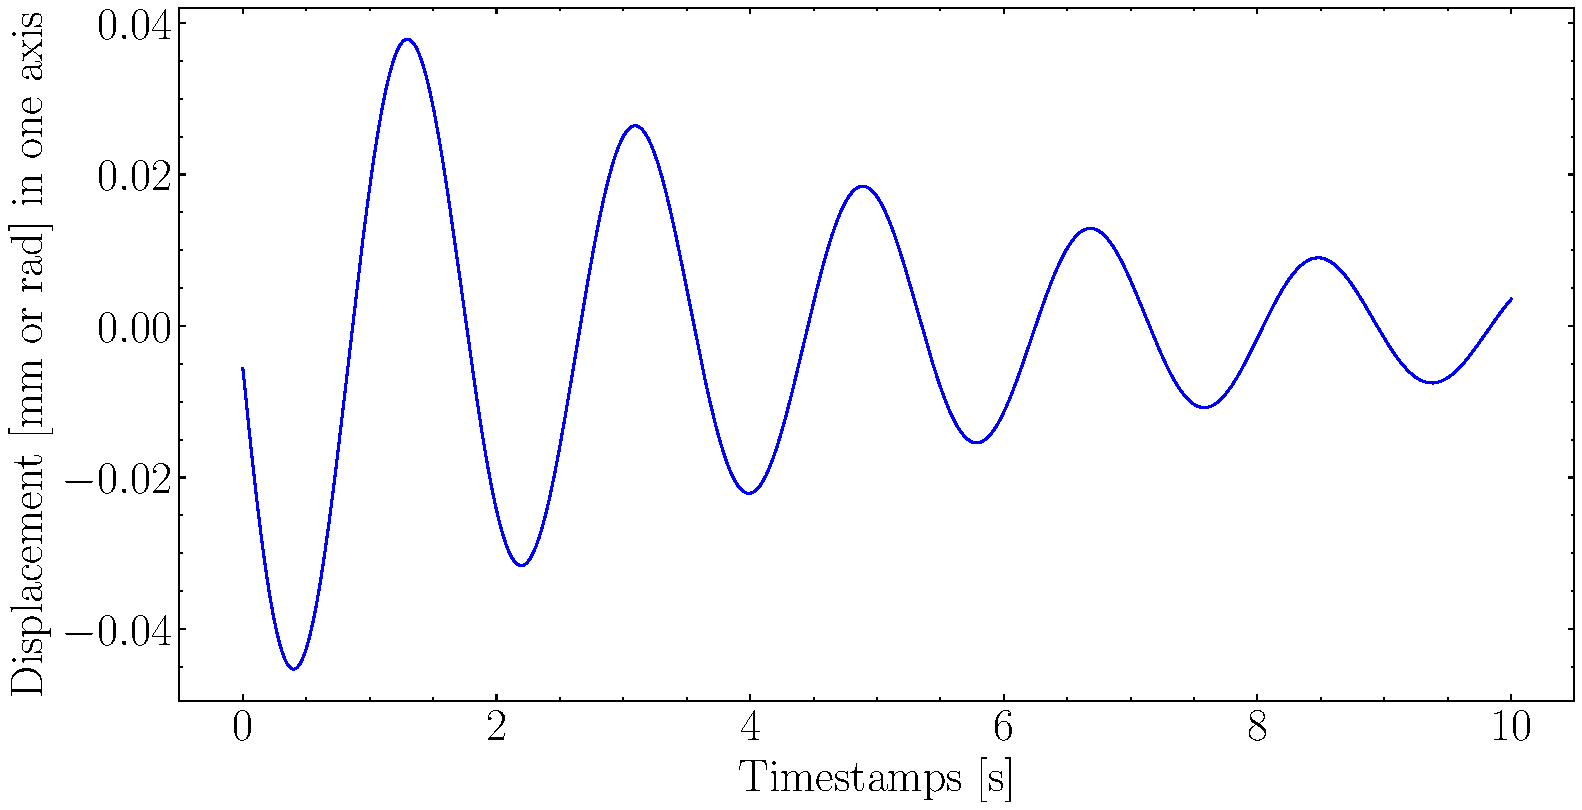
\includegraphics[scale=0.4]{images/fig_chapter4/vib_damped.pdf}
    \caption{Damped vibration in one axis}
    \label{fig:damped_vib}
\end{figure}

%% Displacement distribution
\begin{figure}[H]
    %%
    \begin{subfigure}{\linewidth}
    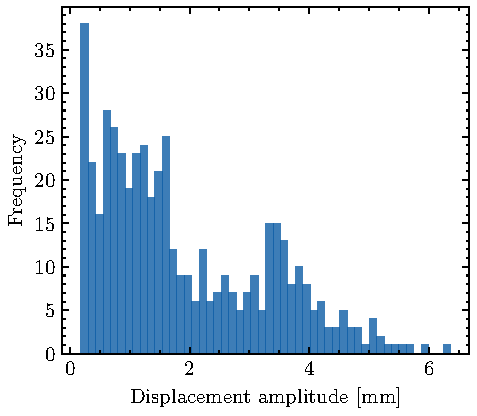
\includegraphics[width=.5\linewidth]{images/fig_chapter4/data_dist/1.pdf}\hfill
    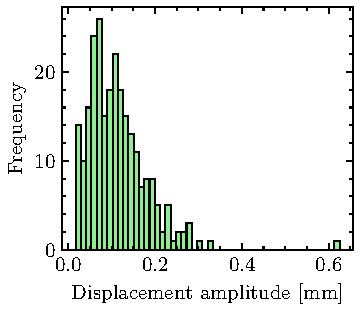
\includegraphics[width=.5\linewidth]{images/fig_chapter4/data_dist/2.pdf}
    \caption{Distribution of maximum translational vibration displacement amplitudes $ A $ in X, Y(left) and Z(right) DoF [mm]}
    \end{subfigure}\par\medskip
    
    %%
    \begin{subfigure}{\linewidth}
    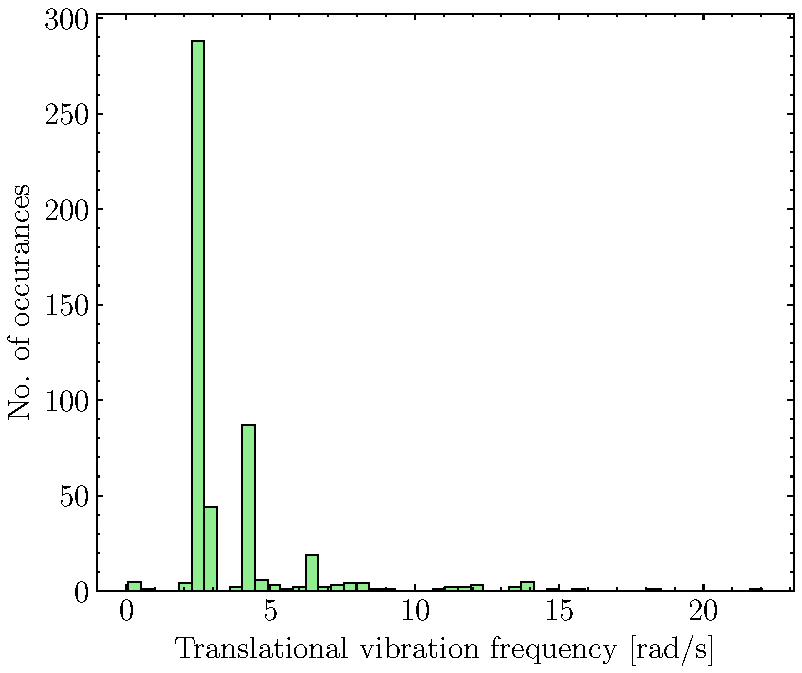
\includegraphics[width=.5\linewidth]{images/fig_chapter4/data_dist/3.pdf}\hfill
    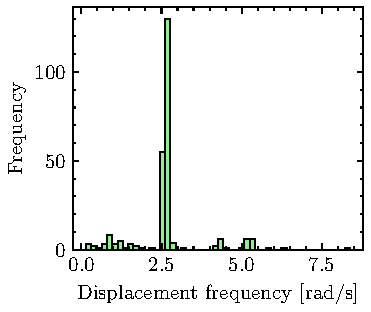
\includegraphics[width=.5\linewidth]{images/fig_chapter4/data_dist/4.pdf}
    \caption{Distribution of translational vibration displacement frequency $ \omega $ in X, Y(left) and Z(right) DoF [mm]}
    \end{subfigure}\par\medskip
    
    %%
    \begin{subfigure}{\linewidth}
    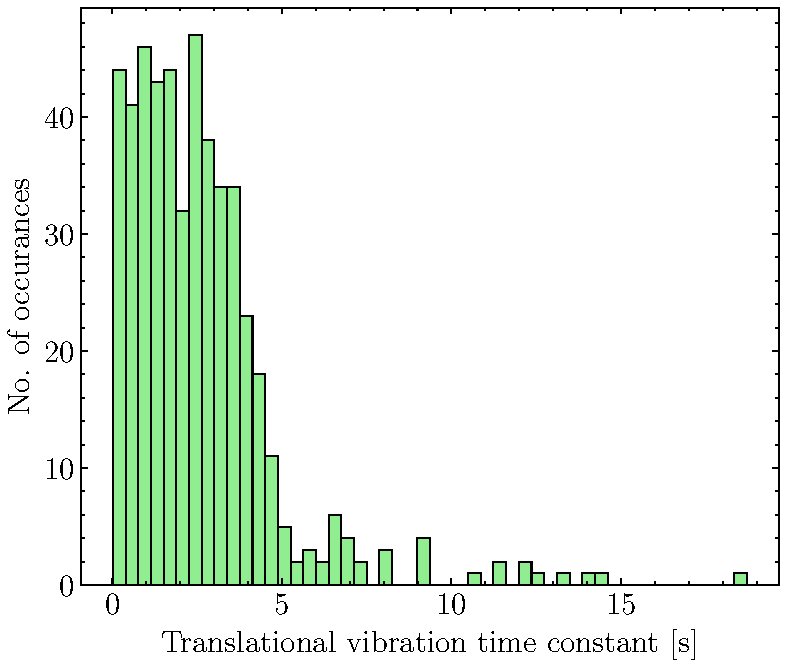
\includegraphics[width=.5\linewidth]{images/fig_chapter4/data_dist/5.pdf}\hfill
    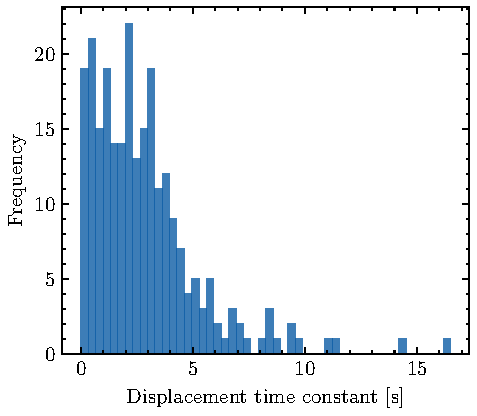
\includegraphics[width=.5\linewidth]{images/fig_chapter4/data_dist/6.pdf}
    \caption{Distribution of translational vibration displacement time-constant $ \tau $ in X, Y(left) and Z(right) DoF [s]}
    \end{subfigure}
\caption{Real translational vibration data statistical analysis}
\label{fig:dist_disp}
\end{figure}

%% Rotation Distribution 
\begin{figure}[H]
    %%
    \begin{subfigure}{\linewidth}
    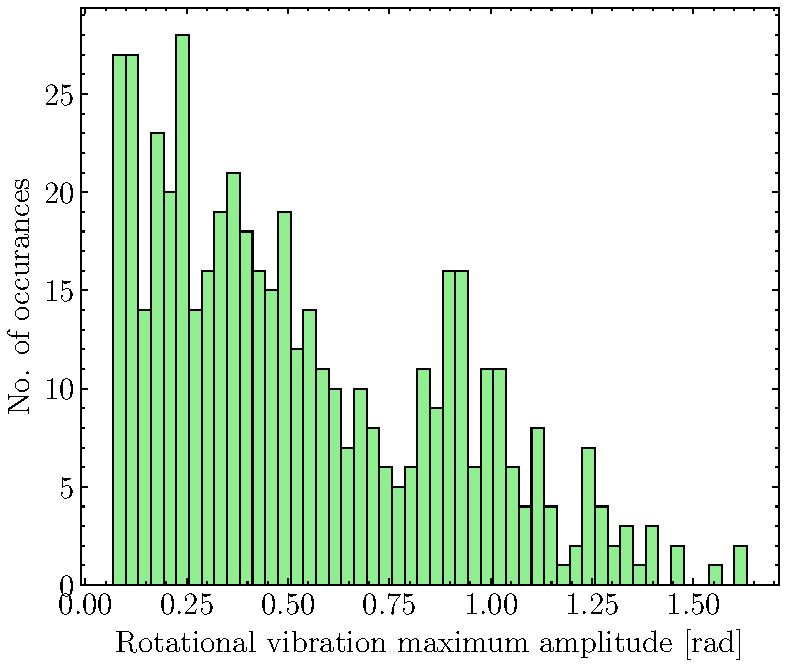
\includegraphics[width=.5\linewidth]{images/fig_chapter4/data_dist/7.pdf}\hfill
    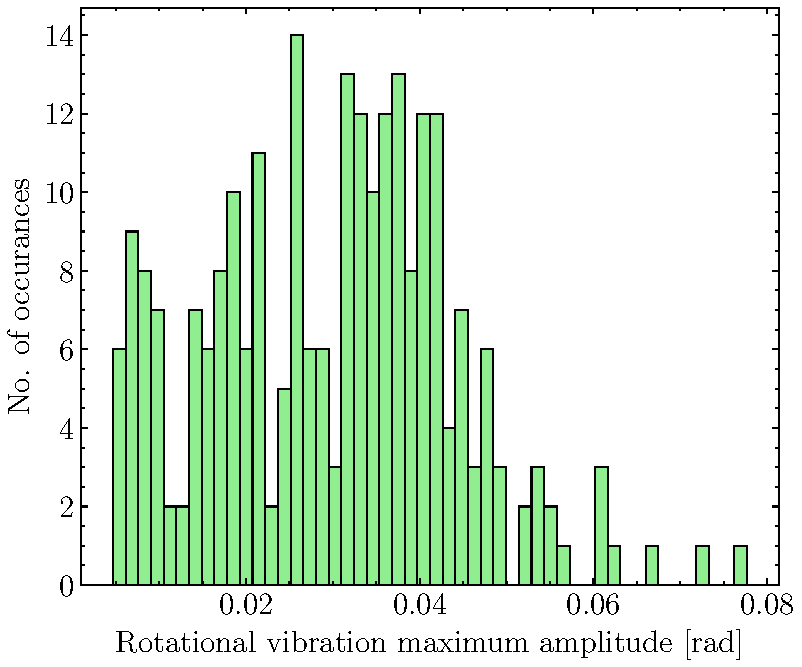
\includegraphics[width=.5\linewidth]{images/fig_chapter4/data_dist/8.pdf}
    \caption{Distribution of rotational vibration displacement amplitude $ \theta $ in X, Y(left) and Z(right) DoF [rad]}
    \end{subfigure}\par\medskip
    
    %%
    \begin{subfigure}{\linewidth}
    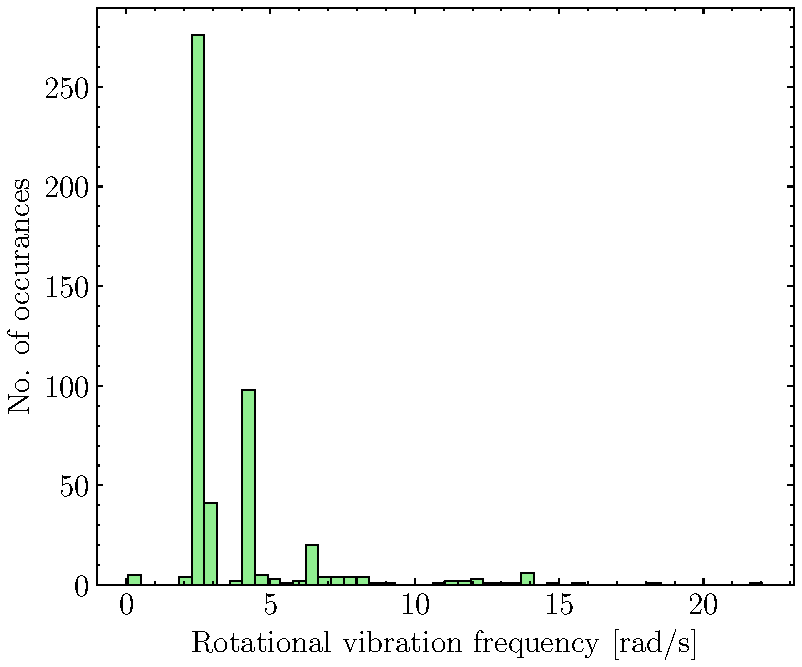
\includegraphics[width=.5\linewidth]{images/fig_chapter4/data_dist/9.pdf}\hfill
    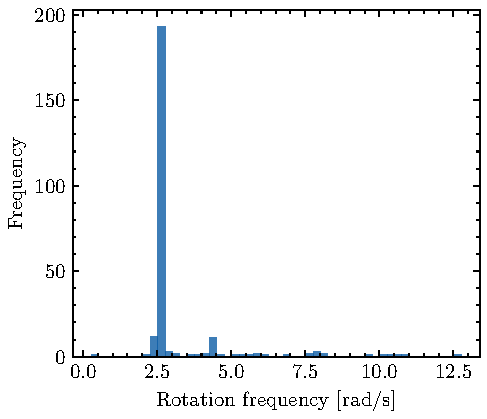
\includegraphics[width=.5\linewidth]{images/fig_chapter4/data_dist/10.pdf}
    \caption{Distribution of rotational vibration displacement frequency $ \omega $ in X, Y(left) and Z(right) DoF [rad/sec]}
    \end{subfigure}\par\medskip
    
    %%
    \begin{subfigure}{\linewidth}
    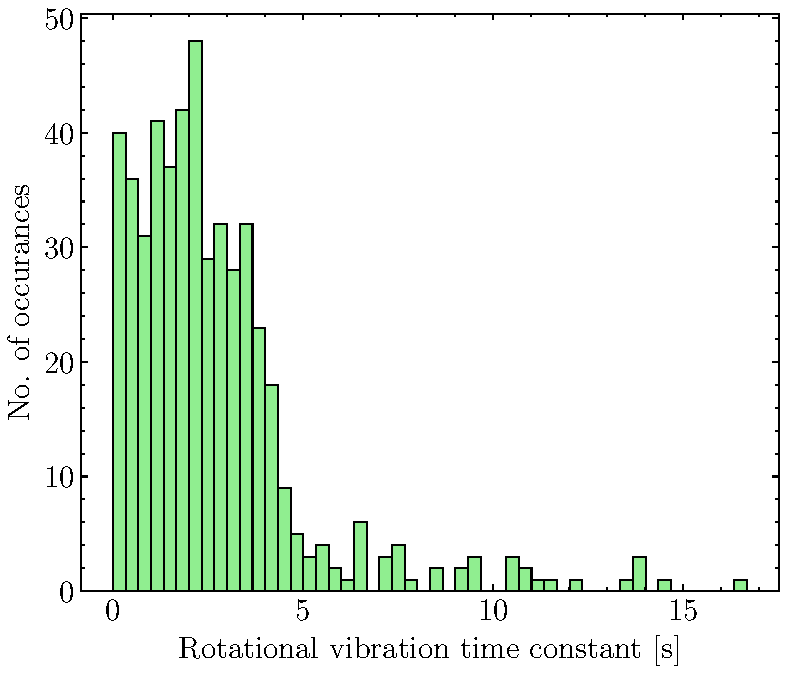
\includegraphics[width=.5\linewidth]{images/fig_chapter4/data_dist/11.pdf}\hfill
    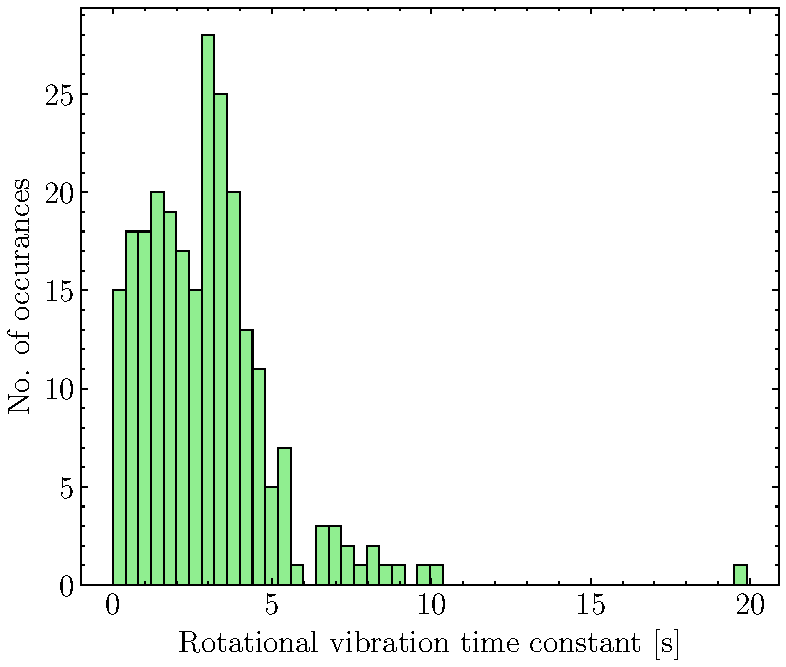
\includegraphics[width=.5\linewidth]{images/fig_chapter4/data_dist/12.pdf}
    \caption{Distribution of rotational vibration displacement time-constant $ \tau $ in X, Y(left) and Z(right) DoF [s]}
    \end{subfigure}

\caption{Real rotational vibration data statistical analysis}
\label{fig:dist_rot}
\end{figure}


The statistical analysis shown in figure \ref{fig:dist_disp} and figure \ref{fig:dist_rot} was done on 248 real world camera setup vibration sequences having an average length of 10 seconds. The results for translational and rotational vibrations are summarised in table \ref{tab:real_data_analysis_displacement} and table \ref{tab:real_data_analysis_rotation} respectively. The rotational vibrations have very small amplitude $ \theta $ and is less than 1 degrees for more than 75 percent of the samples in XY plane. For Z axis the vibrations are even smaller with a mean of 0.0005 degrees. These vibrations are very small and do not have a a noticeable visual effect on the video stabilization. But we have decided to account for them to develop a more general solution with multiple applications. The time constant $ \tau $ for displacement and rotation is similar for all DoF with a mean value of around 2.9 seconds.  The frequency $ \omega $ for all DoF is also similar in the range $ 2.5 rad/sec $ to $ 3.5 rad/sec $. Frequency of $ 2.5 rad/sec $ is the most dominant frequency and seems to be the natural frequency $ \omega_n $ of the mechanical system (camera setup).


The amplitude $ A $ of the translational displacements is the most important characteristic as it is main source of video destabilization. The effect of motion on the quality of video is more pronounced in XY plane as the most pixel shift happens here. In Z axis the mean $ \mu $ of translational vibrations is 0.113 mm with a standard deviation ($ \sigma^{2} $) of 0.07 mm. Even the large displacements in Z seem to have little effect on visual quality of the video. Transnational vibration displacements in XY plane have the mean of 1.9 mm with a standard deviation of 1.36 mm. Vibrations with higher magnitude are also present and need to be accounted for when generating simulated data.

% displacement data distribution table
\begin{table}[H]
    \centering
\begin{tabular}{ c | L | L | L }
    
     Parameter  & 
     Mean ($ \mu $) & 
     Variance ($ \sigma^{2} $) &
     Standard Deviation ($ \sigma $)\\
     \hline
     
     $ A_{xy} $ & 
     $ 1.89 mm $ & 
     $ 1.86 mm^{2} $ &
     $ 1.36 mm $ \\

      
     $ A_{z} $  & 
     $ 0.11 mm $ & 
     $ 0.0047 mm^{2} $ &
     $ 0.06 mm $ \\
     
     
     $ \omega_{xy} $ & 
     $ 3.68 rad/s $ & 
     $ 5.98 rad^{2}/s^{2} $ &
     $ 2.44 rad/s $ \\
     
     
     $ \omega_{z} $& 
     $ 2.68 rad/s $ & 
     $ 2.07 rad^{2}/s^{2} $ &
     $ 1.03 rad/s $ \\

     
     $ \tau_{xy} $ & 
     $ 2.59 s $ & 
     $ 5.18 s^{2} $ &
     $ 2.27 s $ \\


     $ \tau_{z} $ & 
     $ 2.83 s $ & 
     $ 5.87 s^{2} $ &
     $ 2.42 s $ \\

\end{tabular}
    \caption{Real translational-vibration data distributions}
    \label{tab:real_data_analysis_displacement}
\end{table}

% rotation data distribution table
\begin{table}[H]
    \centering
\begin{tabular}{ c | L | L | L }

     Parameter  & 
     Mean ($ \mu $) & 
     Variance ($ \sigma^{2} $) &
     Standard Deviation ($ \sigma $)\\
     \hline
     
     $ \theta_{xy} $ & 
     $ 0.0094 rad $ & 
     $ 3.87e^{-8} rad^{2} $ &
     $ 0.0062 rad $ \\

      
     $ \theta_{z} $  & 
     $ 0.0005 rad $ & 
     $ 6.07e^{-8} rad^{2} $ &
     $ 0.0002 rad $ \\
     
     
     $ \omega_{xy} $ & 
     $ 3.80 rad/s $ & 
     $ 6.36 rad^{2}/s^{2} $ &
     $ 2.52 rad/s $ \\

     
     $ \omega_{z} $& 
     $ 3.17 rad/s $ & 
     $ 2.62 rad^{2}/s^{2} $ &
     $ 1.61 rad/s $ \\
   
     
     $ \tau_{xy} $ & 
     $ 2.65 s $ & 
     $ 5.83 s^{2} $ &
     $ 2.41 s $ \\
    
     
     $ \tau_{z} $ & 
     $ 2.93 s $ & 
     $ 4.73 s^{2} $ &
     $ 2.17 s $ \\

\end{tabular}
    \caption{Real rotational-vibration data distributions}
    \label{tab:real_data_analysis_rotation}
\end{table}



\subsection{Simulated Data Generation}
\label{sec:gen_sim_data}
The simulated data plays a very important role in our approach as we use the ideal data to validate our stabilization approach. It also empowers us to simulate IMU sensors with different noise levels and characteristics. We also made sure that the data generated from the simulation is fairly domain randomized to make it realistic. 

Simulated data is based on the analysed real data with vibration characteristics taken from table \ref{tab:real_data_analysis_displacement} and table \ref{tab:real_data_analysis_rotation}. The data is then generated using the equations \ref{eqn:vib_disp} and \ref{eqn:vib_rot}. A total of 400 vibration sequences with an average vibration duration of 10 seconds were generated with characteristics shown in tables \ref{tab:real_data_analysis_displacement} and \ref{tab:real_data_analysis_rotation}. Generating a large number of samples ensures the sampling of diverse data from the distribution. This is where we benefit from our simulation the most as the diversity and the size of data ensures our neural network generalizes well.


\section{Structuring of Data}
\label{sec:data_structure}
In classical pose-estimation techniques, every single IMU sample is integrated to the pose estimation individually. Data driven approaches differ in this case as discussed in section \ref{sec:sota_pose_est}. For data driven approaches instead of taking an individual sample a \textit{window} of samples (figure \ref{fig:imu_window_samples}) is used as a single sample does not contain enough information to extract meaningful information. 

In a supervised learning setting, neural networks require a sufficient amount of data to prevent them from over-fitting to a few samples and to be able to learn the underlying statistics and patterns in the data. Initially we experimented with small window samples (3 - 20 samples) as shown in figure \ref{fig:imu_window_samples} a. This did not yield very good results and the pose estimation error was too high for accurate stabilization. Good results were achieved with window a window size between 70 to 150 samples (example of windows of IMU data depicted in figure \ref{fig:imu_window_samples}). Larger window sizes did not have an influence on the accuracy but led to increased inference times of the neural network and latency became too high. Hence in the following a window size of 143 was chosen.

\begin{figure}[H]
    %%
    \begin{subfigure}{\linewidth}
    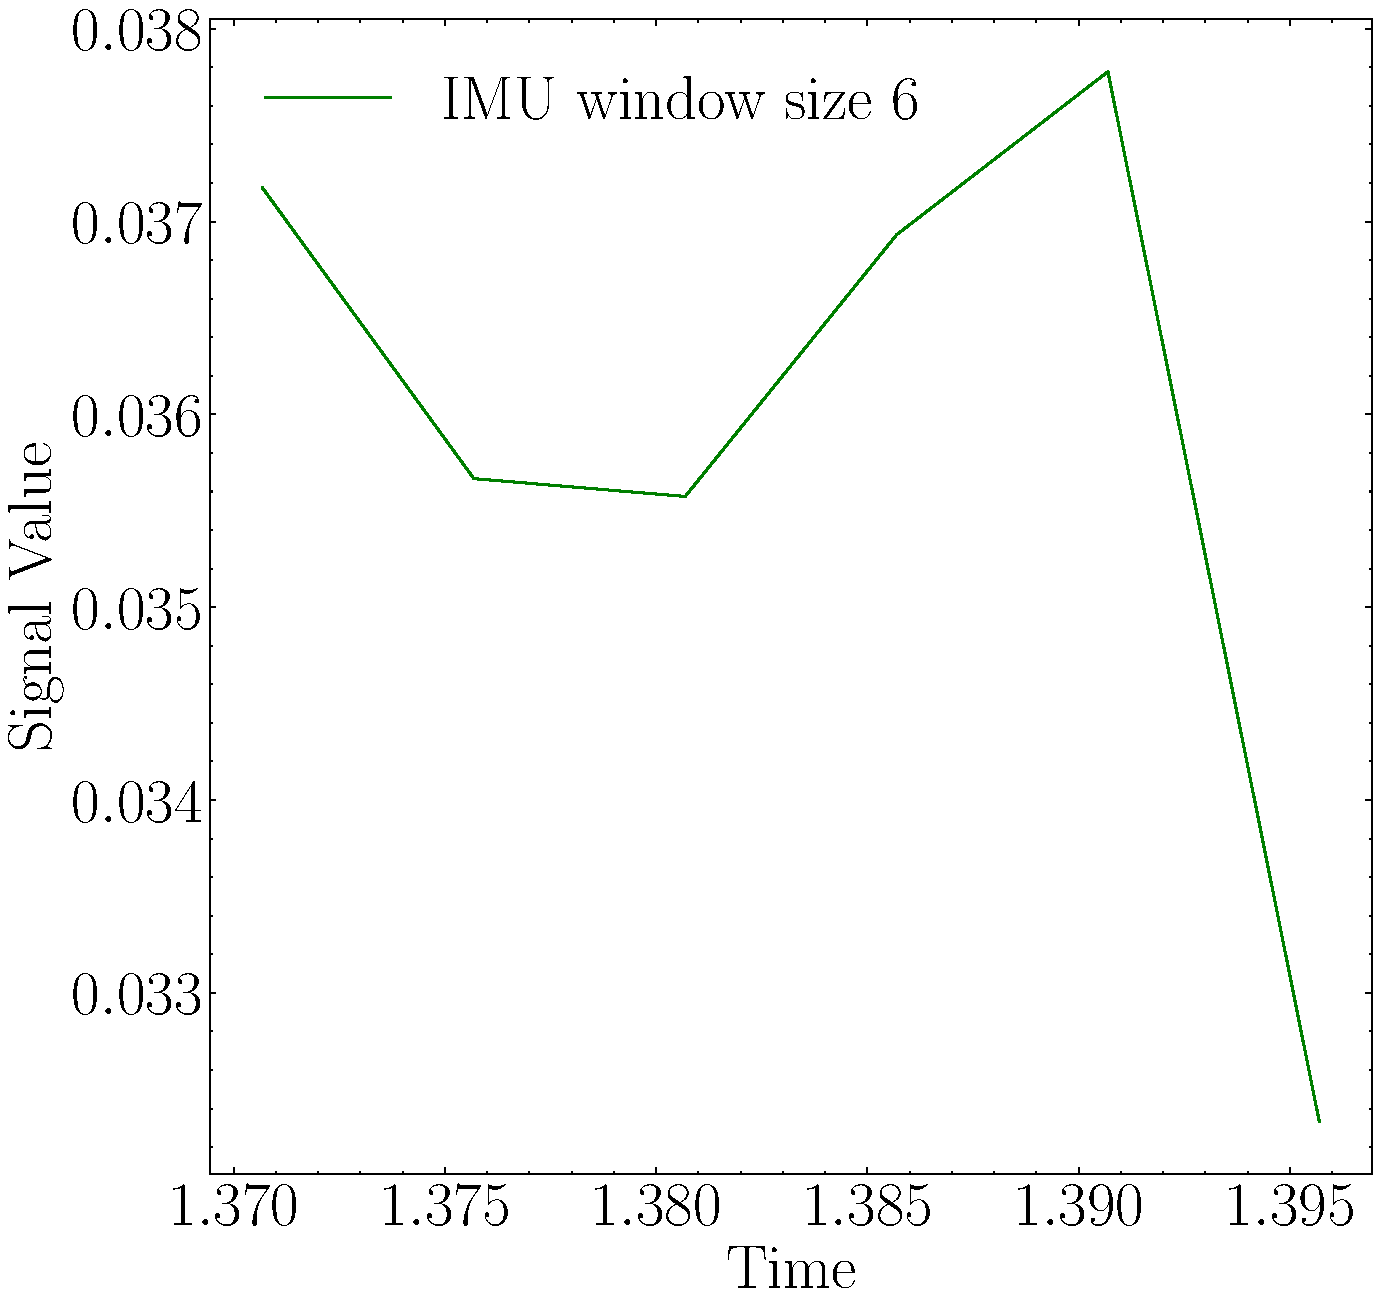
\includegraphics[width=.3\linewidth]{images/fig_chapter4/imu_windows/imu_window_size_6.pdf}\hfill
    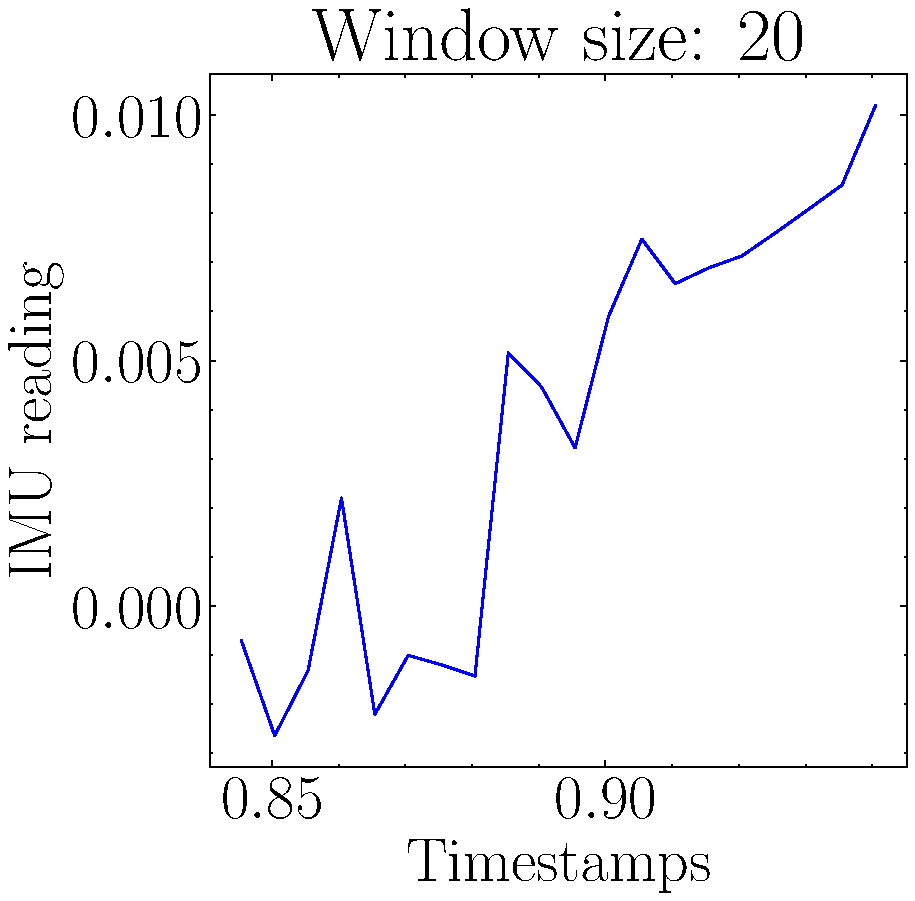
\includegraphics[width=.3\linewidth]{images/fig_chapter4/imu_windows/imu_window_size_20.pdf}\hfill
    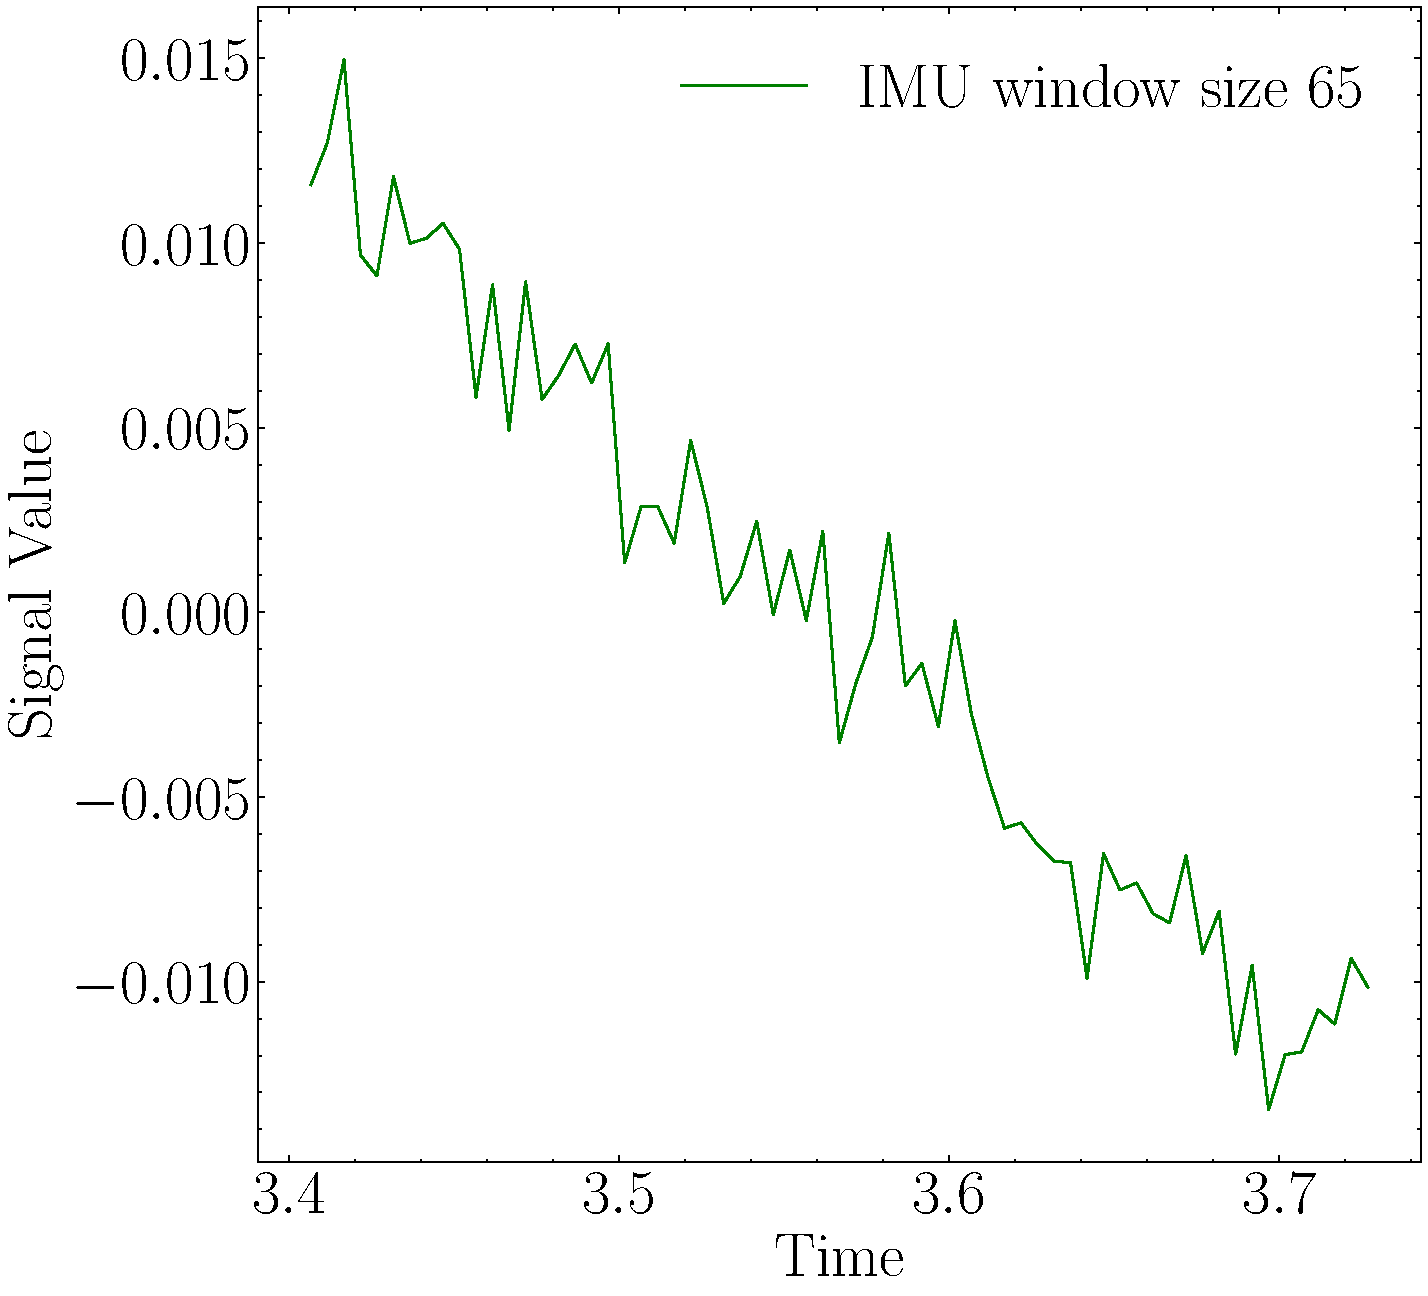
\includegraphics[width=.3\linewidth]{images/fig_chapter4/imu_windows/imu_window_size_65.pdf}\hfill
    \caption{Window size 6, 20 and 65}
    \end{subfigure}\par\medskip
    
    %%
    \begin{subfigure}{\linewidth}
    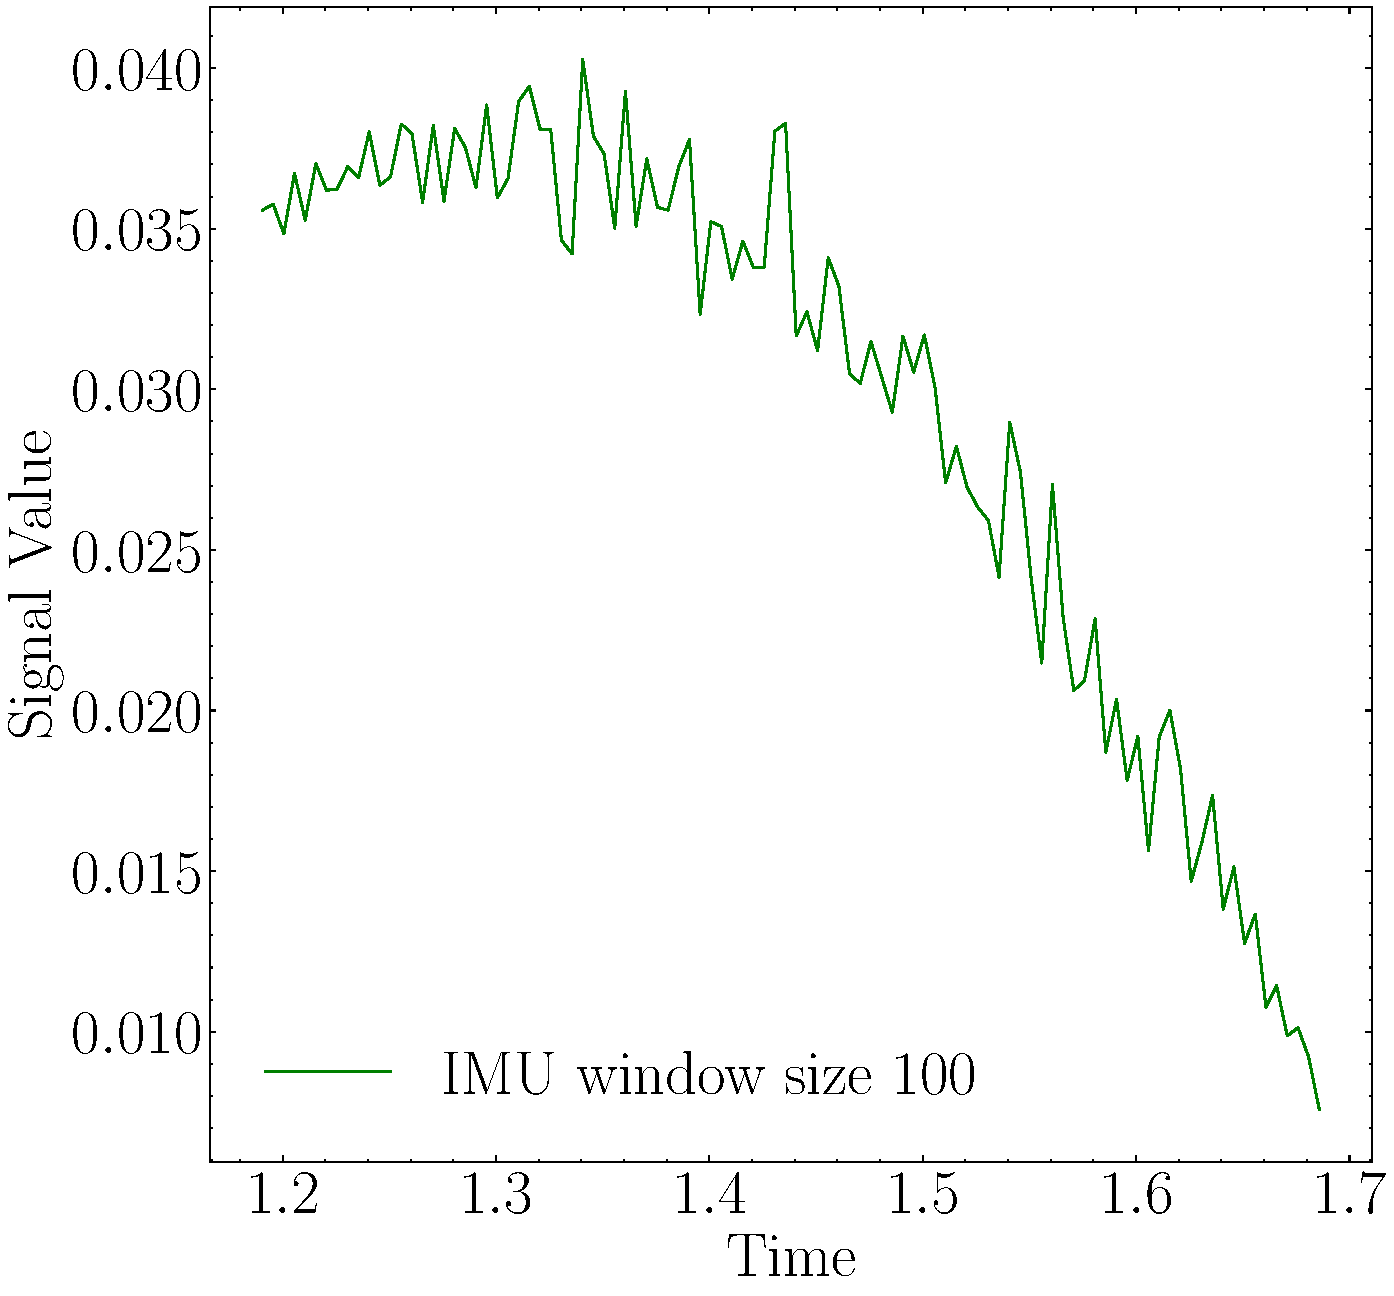
\includegraphics[width=.3\linewidth]{images/fig_chapter4/imu_windows/imu_window_size_100.pdf}\hfill
    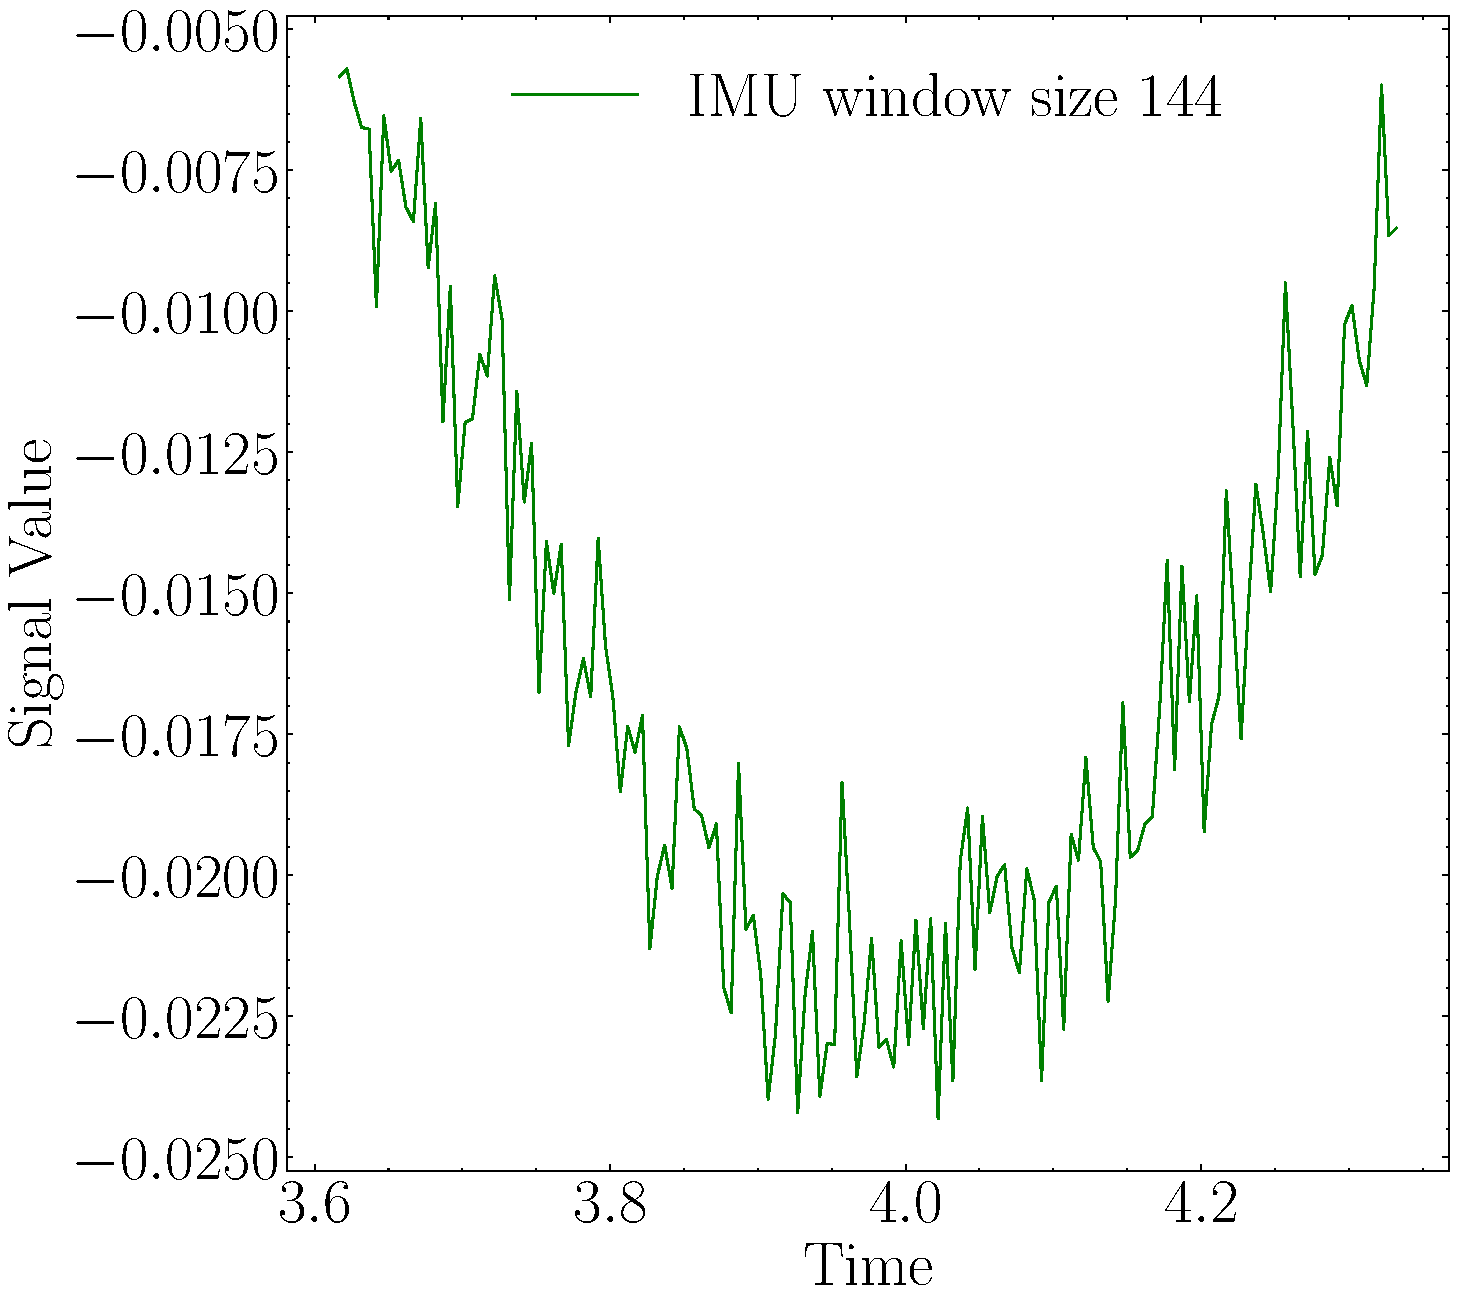
\includegraphics[width=.3\linewidth]{images/fig_chapter4/imu_windows/imu_window_size_144.pdf}\hfill
    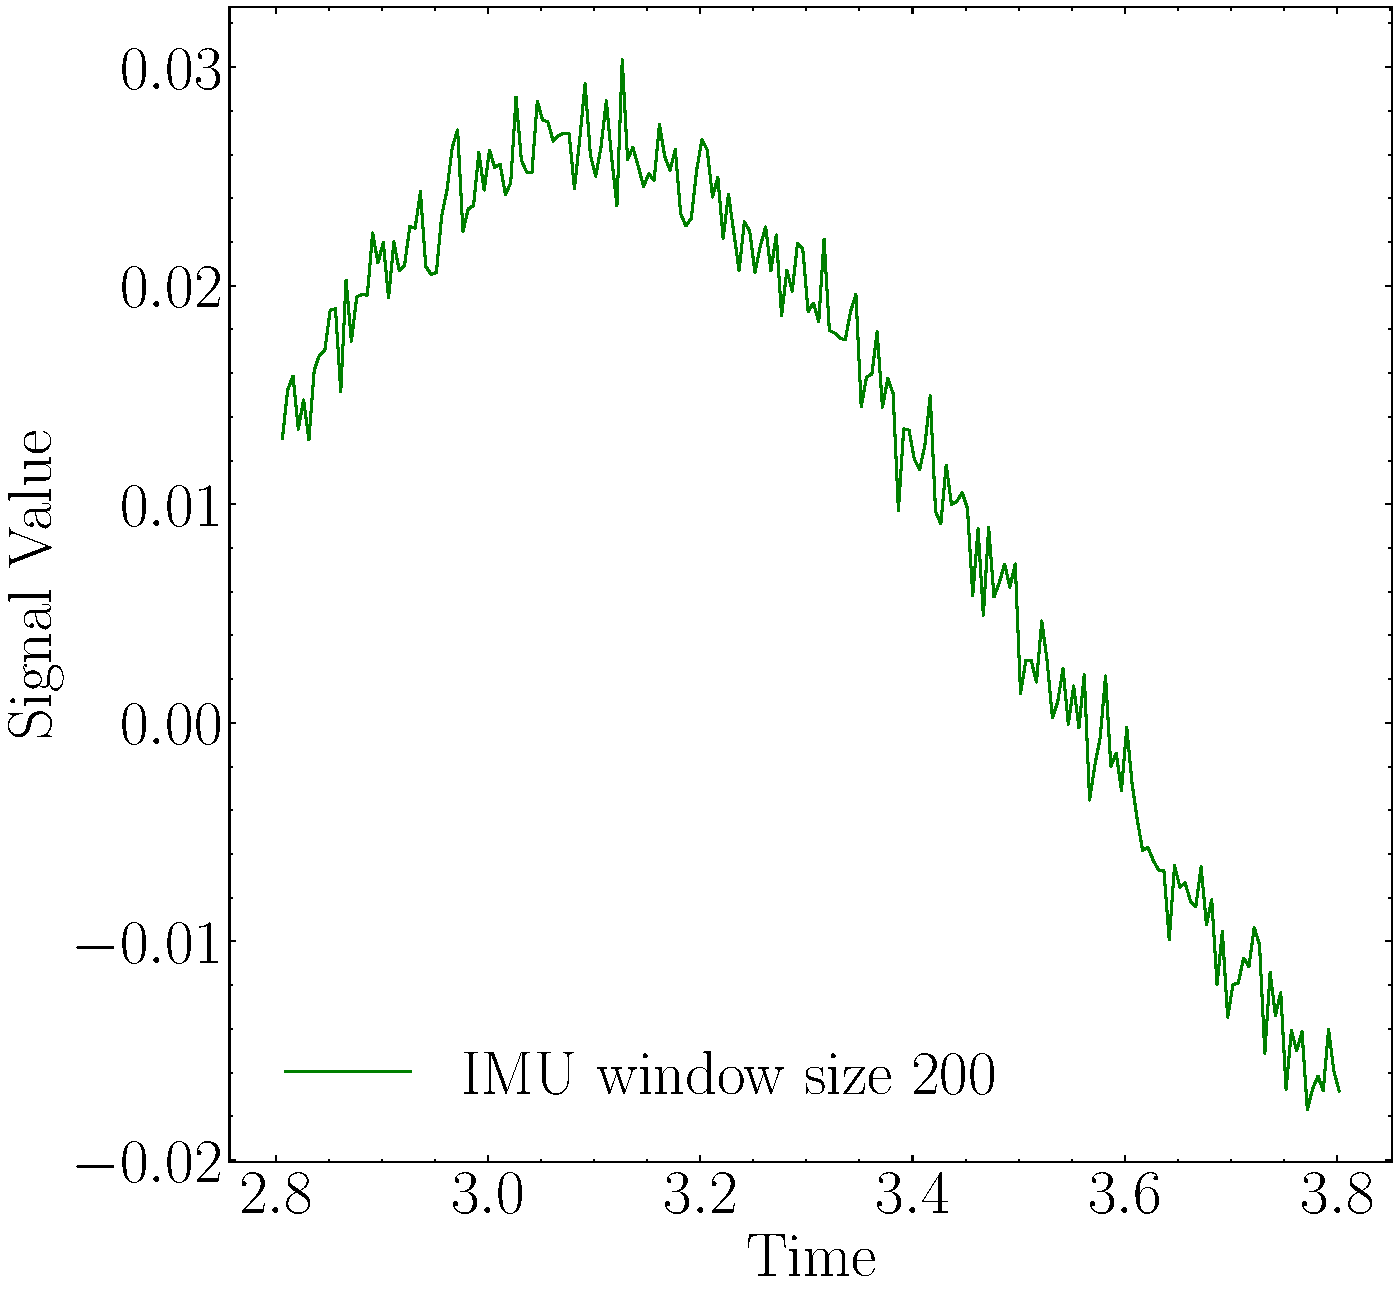
\includegraphics[width=.3\linewidth]{images/fig_chapter4/imu_windows/imu_window_size_200.pdf}\hfill
    \caption{Window size 100, 144, 200}
    \end{subfigure}
\caption{Different IMU window samples}
\label{fig:imu_window_samples}
\end{figure}

\section{Training and Testing of Various Neural Networks}
Various neural network architectures were trained and tested to accurately estimate the camera pose with respect to a stabilized trajectory. The input to the neural network is a window of sensor readings coming from an IMU and the network is trained against the deviation with respect to the stabilization trajectory. The stabilization trajectory can be realised as a mean of the vibration displacement (linear/angular) for an ideal case as shown in figure \ref{fig:stab_traj_ideal}. 

\begin{figure}
    \centering
    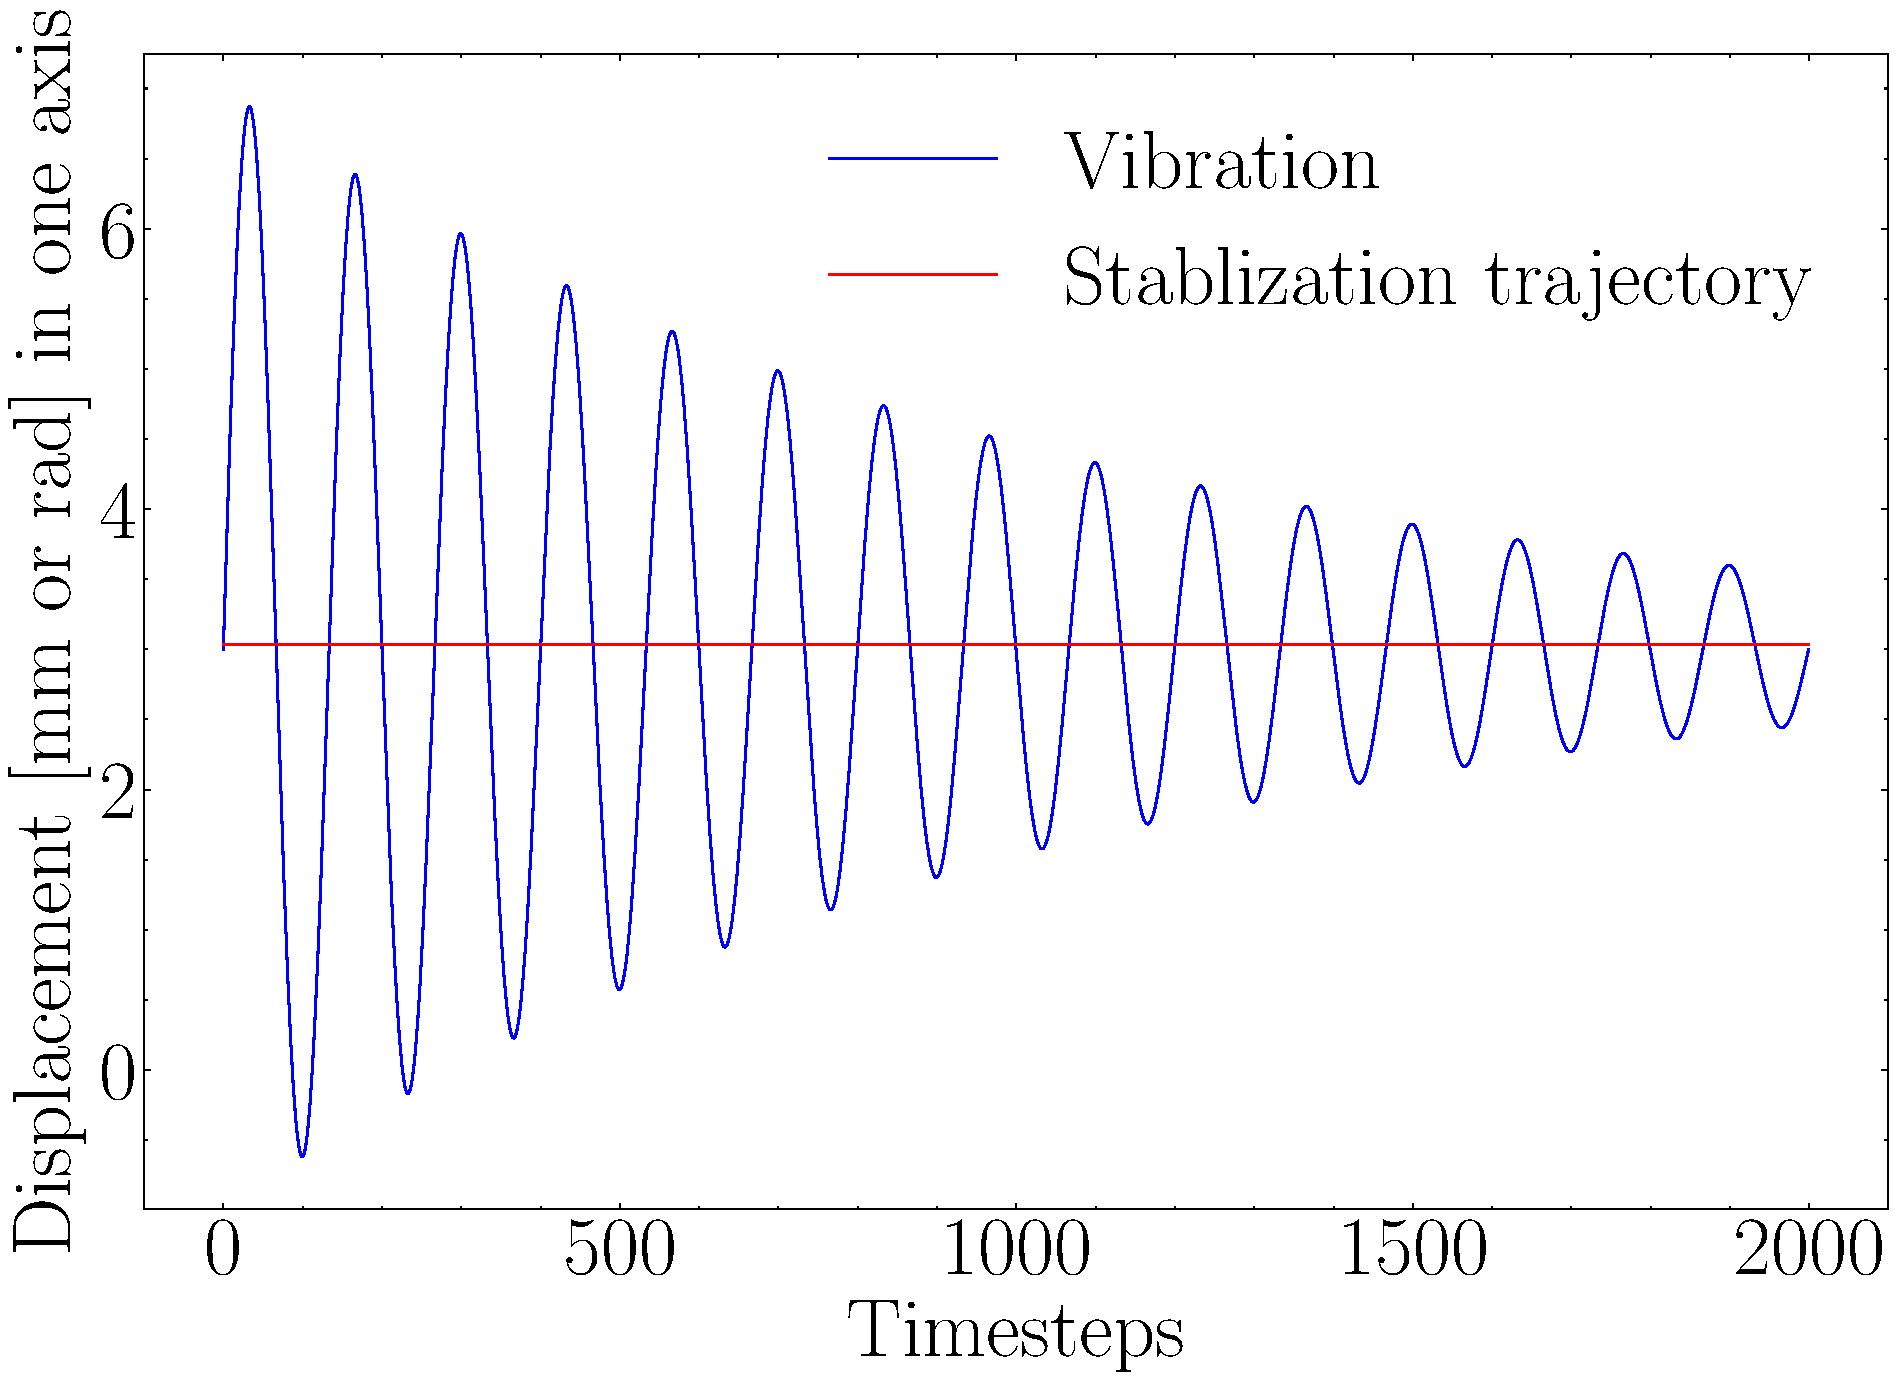
\includegraphics[scale=0.25]{images/fig_chapter2/stab_traj_ideal.pdf}
    \caption{Stabilization trajectory (Ideal)}
    \label{fig:stab_traj_ideal}
\end{figure}

Let the variable window size be \textbf{W}. Then based on the employed sensor data (either only accelerometer or accelerometer + gyroscope) the input size to the network is either (3,W) or (6,W) respectively. The use of accelerometer readings is a must because destabilization caused in our use case is mostly due to translational displacements as discussed in chapter section \ref{sec:data_analysis}. 

Various neural network architectures like CNN, MLP, LSTM, ResNet, Transformers and their variations were trained and tested for stabilization trajectory regression. Out of these CNN, ResNet and Transformer architectures had acceptable performance. 

\subsection{Data Augmentation}
The simulated data is augmented with modified noise and bias characteristics from table \ref{tab:imu_noise_characteristics}. On each training step randomly generated bias and white noise is added to the true IMU window samples. This results in the network learning to compensate for white noise and bias for a wide variety of noise characteristics as shown by the decrease of average trajectory error by 5 percent.

\subsection{Training Setting}
The training dataset consists of 400 samples of length 10 seconds each. Which means a total of more than 5000 IMU windows \textit{W} of size (6, 143) are available for training, validation and testing the network. The training, validation and testing had a split of 80:15:5. The network was trained using the Adam optimizer with an initial learning rate of 1x$ 10^{-5} $ and a learning rate scheduler. Initial learning rate was estimated with PyTorch-Lighting and optimized using grid search. Mean Squared Error (MSE) proved to be the best loss function for this use case and is also used by other data driven pose estimation algorithms \citep{yan2018ridi}, \citep{herath2020ronin}.

\textbf{Note}: In the next sections, only output plots for translational displacement predictions will be shown as as the rotation is very small and all the networks correctly predict it with average error in micro-radians range.

%% CNN
\subsection{Convolutional Neural Network}
A convolutional neural network with six stacked Conv1D layers each with batch normalization and ReLU activations is used to extract features from the input data as shown in figure \ref{fig:cnn_used}. Then the output of these convolution layers is regularized during training using \textbf{dropout} and down-sampled using \textbf{Max-pooling}. Finally, pose is regressed using a series of two fully connected \textbf{MLP} layers.

\begin{figure}
    \centering
    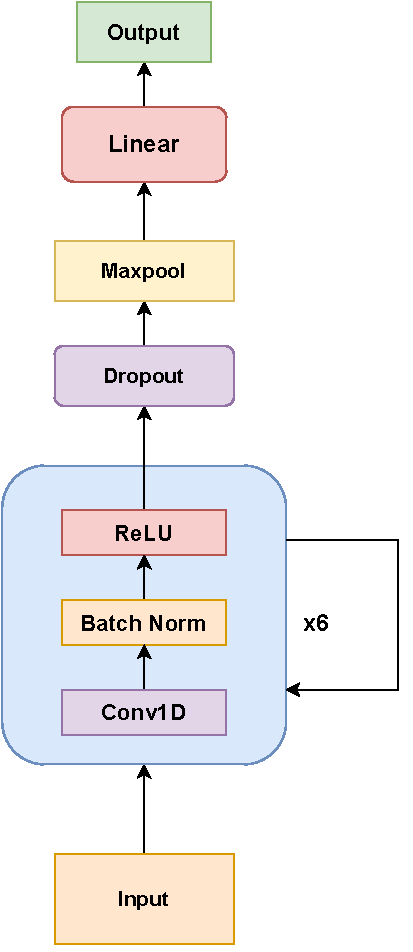
\includegraphics[scale=0.75]{images/fig_chapter2/nns/cnn_mt.pdf}
    \caption{Convolutional Neural Network used}
    \label{fig:cnn_used}
\end{figure}

\subsubsection{Model Output Analysis}
Figure \ref{fig:cnn_op_vs_gt} shows the model output vs ground truth plot for a 27 seconds long video with translational vibrations in 3 axis (x,y,z). The model can regress stabilization trajectory based on input IMU readings with good precision but there are zones where the prediction too far off and not smooth enough which will case jitter in the stabilization. The error in all axis is depicted in figure \ref{fig:cnn_error}.

\begin{figure}[H]
    \centering
    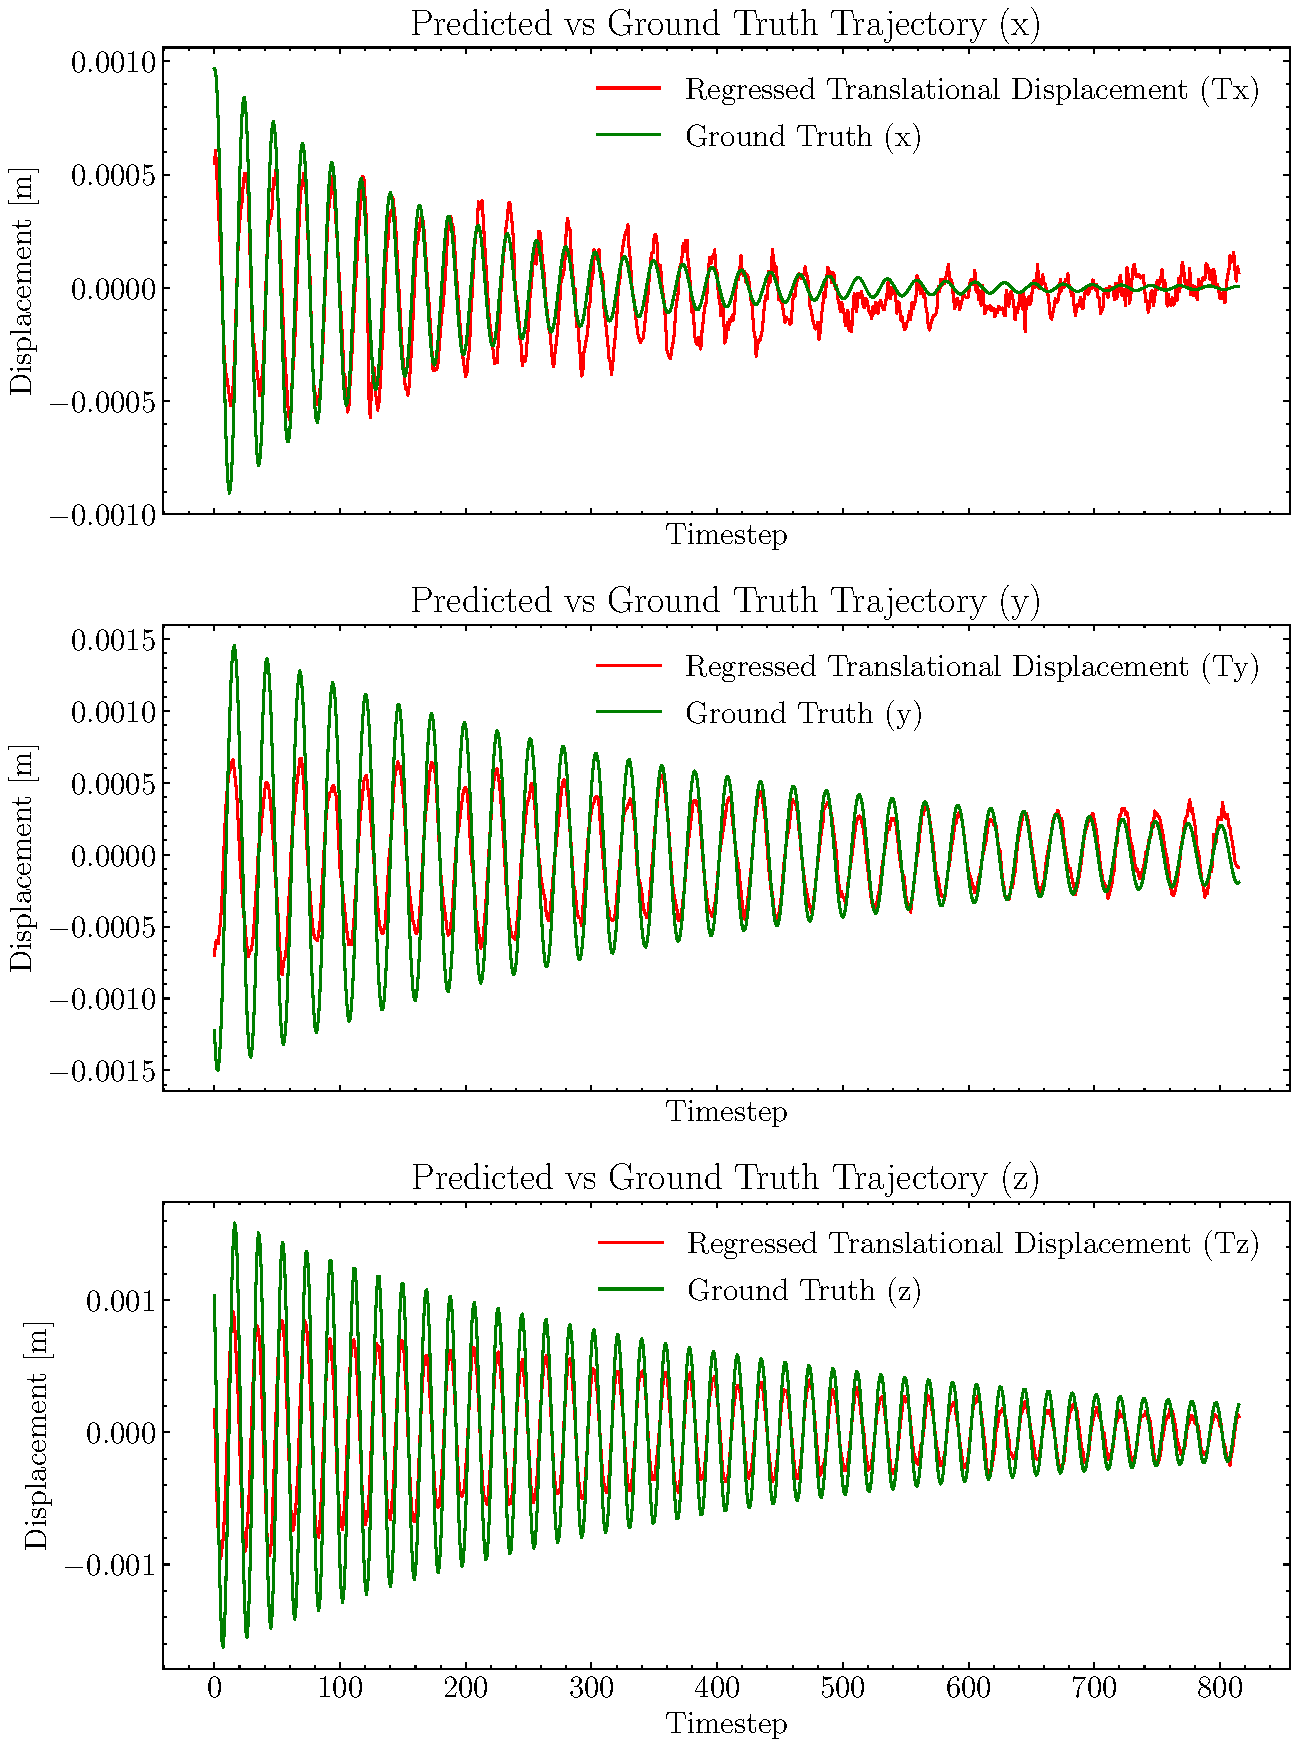
\includegraphics[scale=0.53]{images/fig_chapter4/nn_related/predicted_vs_ground_truth_cnn.pdf}
    \caption{Model prediction vs ground truth for CNN}
    \label{fig:cnn_op_vs_gt}
\end{figure}

\begin{figure}[H]
    \centering
    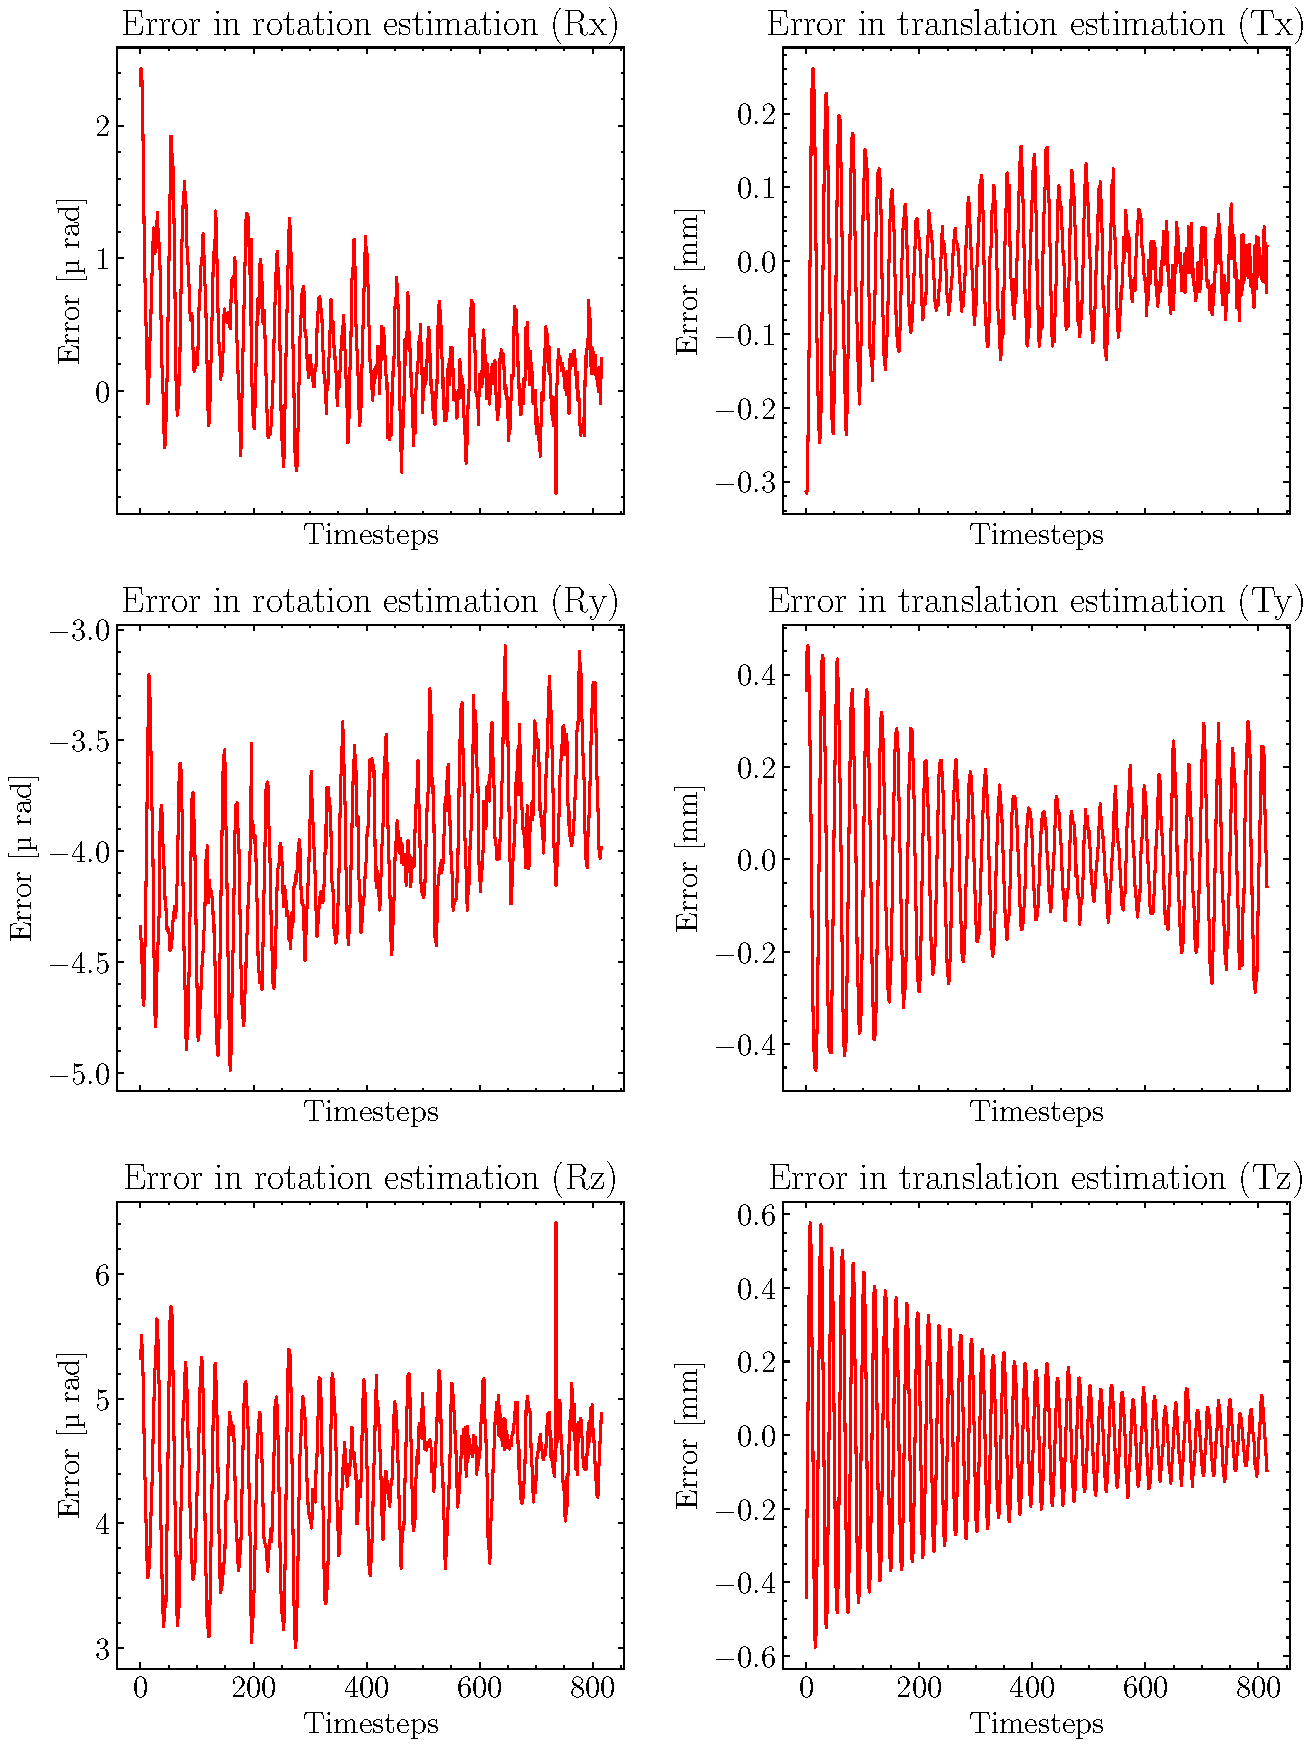
\includegraphics[scale=0.5]{images/fig_chapter4/nn_related/error_in_predicted_vs_ground_truth_cnn.pdf}
    \caption{Error in each axis for CNN}
    \label{fig:cnn_error}
\end{figure}

%% ResNet
\subsection{ResNet}
Convolution neural network having \textbf{Residual Skip Connections} with six \textbf{1D-Convolutional} Layers in sequence with \textbf{Batch Normalisation} and  \textbf{ReLU} activation is used to extract features from the input data. Then the output of these convolution layers is regularized using \textbf{dropout} and down-sampled using \textbf{Max-pooling}. Finally, pose is regressed using a series of two fully connected \textbf{Linear} layers. 

\subsubsection{Model Output Analysis}
Figure \ref{fig:resnet_op_vs_gt} shows the model output vs ground truth plot for a 27 seconds video three linear DoF (x, y, z). The model can regress stabilization trajectory based on input IMU readings with good precision but there are zones where the prediction is off and thus causes jitter in stabilization. The error in all DoF can be seen in figure \ref{fig:resnet_error}.

\begin{figure}[H]
    \centering
    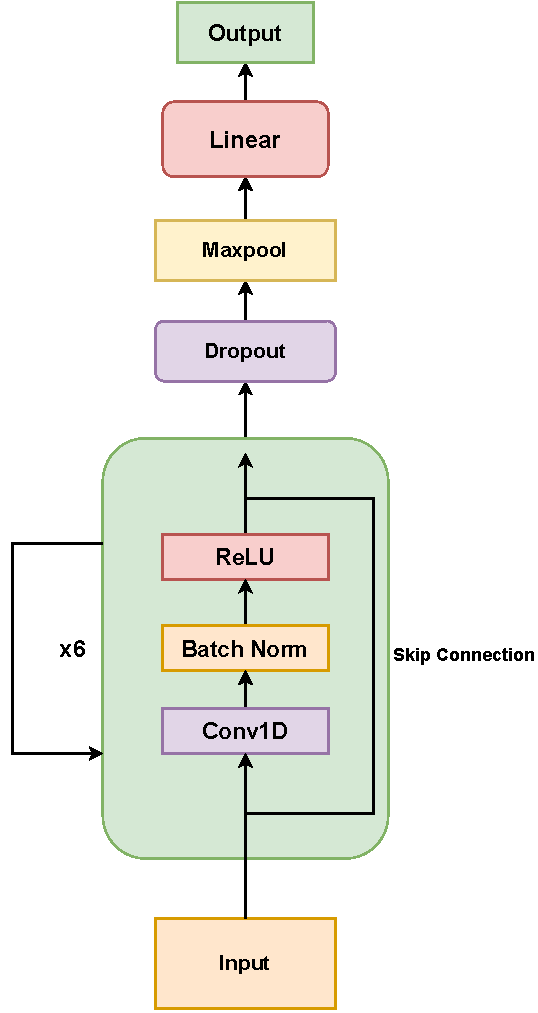
\includegraphics[scale=0.55]{images/fig_chapter2/nns/resnet_mt.pdf}
    \caption{CNN with residual skip connections (ResNet)}
    \label{fig:resnet_used}
\end{figure}

\begin{figure}[H]
    \centering
    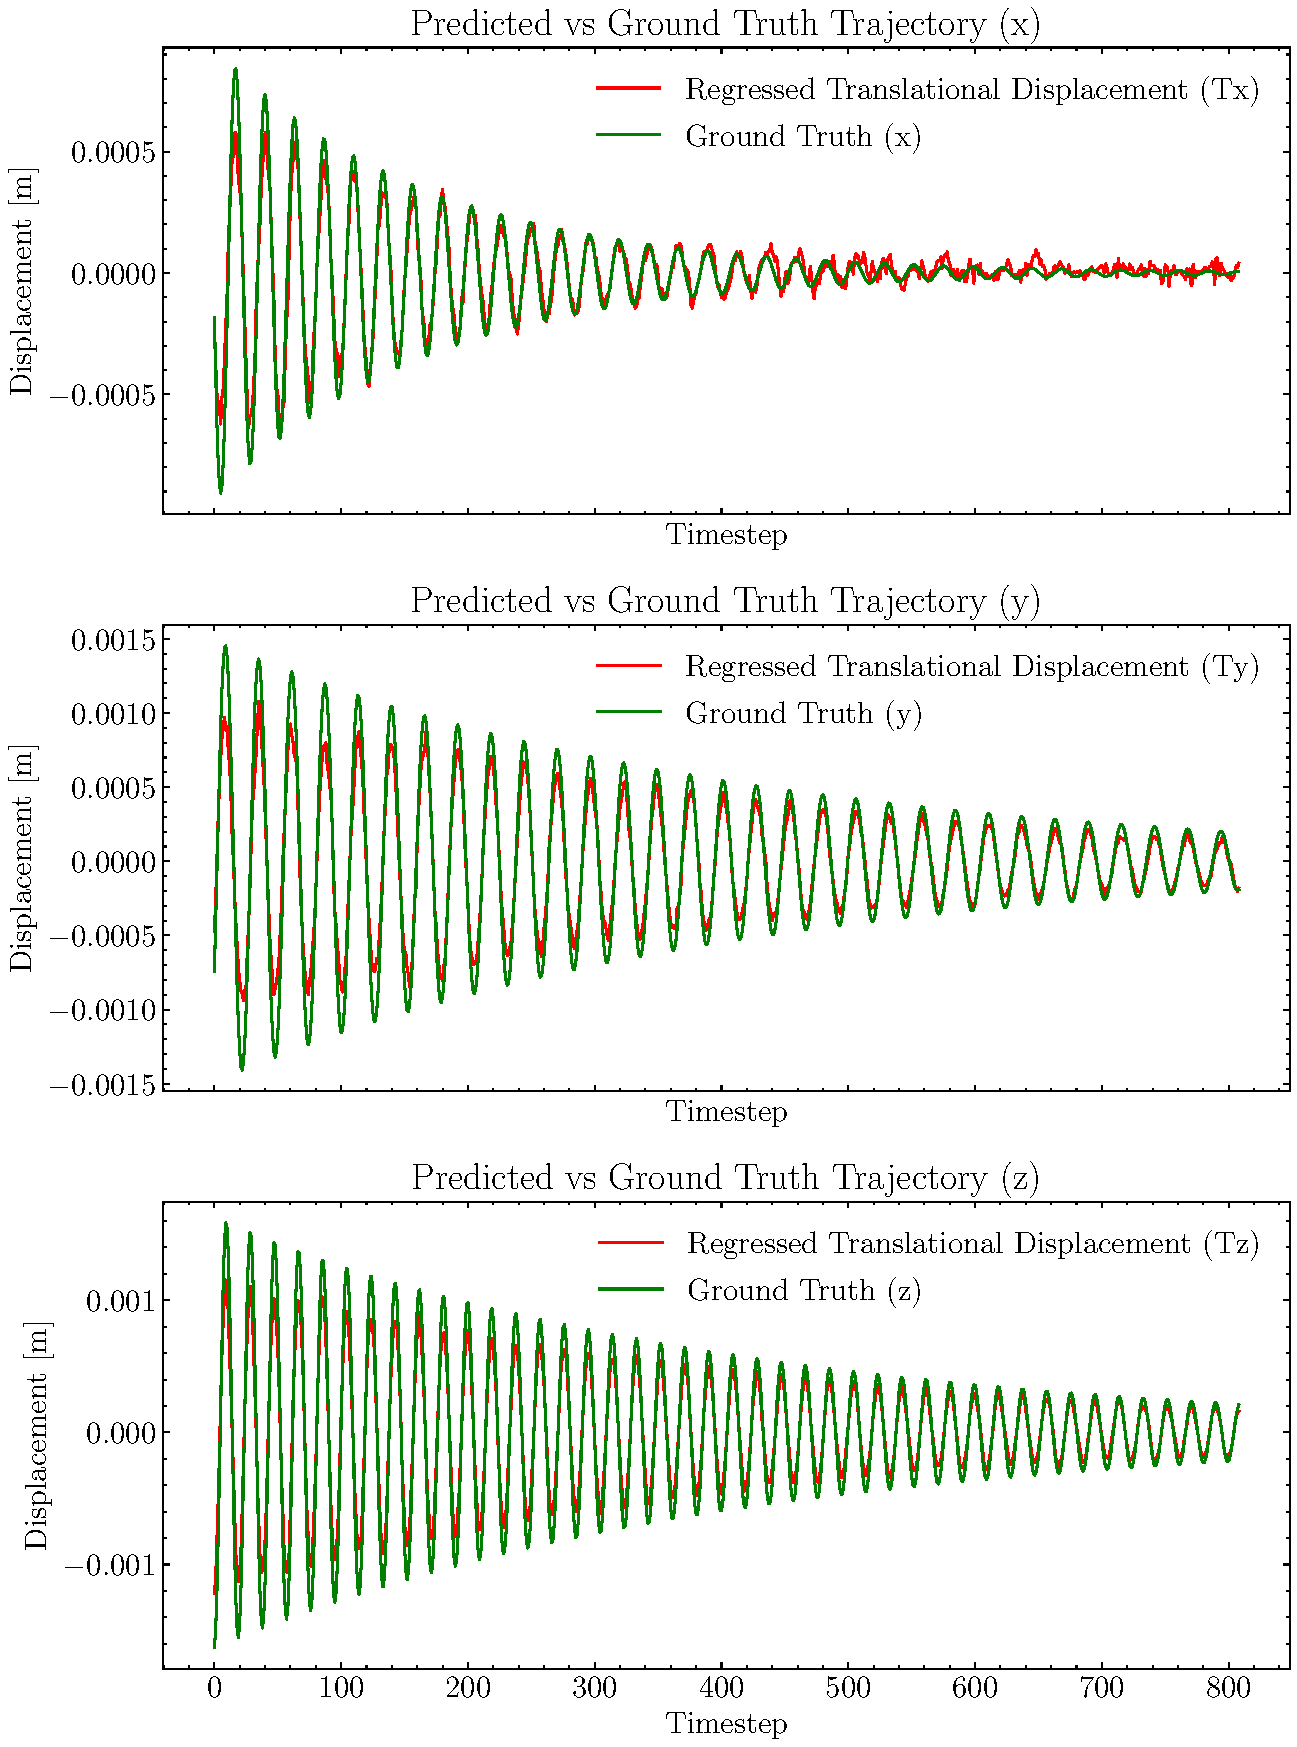
\includegraphics[scale=0.6]{images/fig_chapter4/nn_related/predicted_vs_ground_truth_resnet.pdf}
    \caption{Model prediction vs ground truth for ResNet}
    \label{fig:resnet_op_vs_gt}
\end{figure}

\begin{figure}[H]
    \centering
    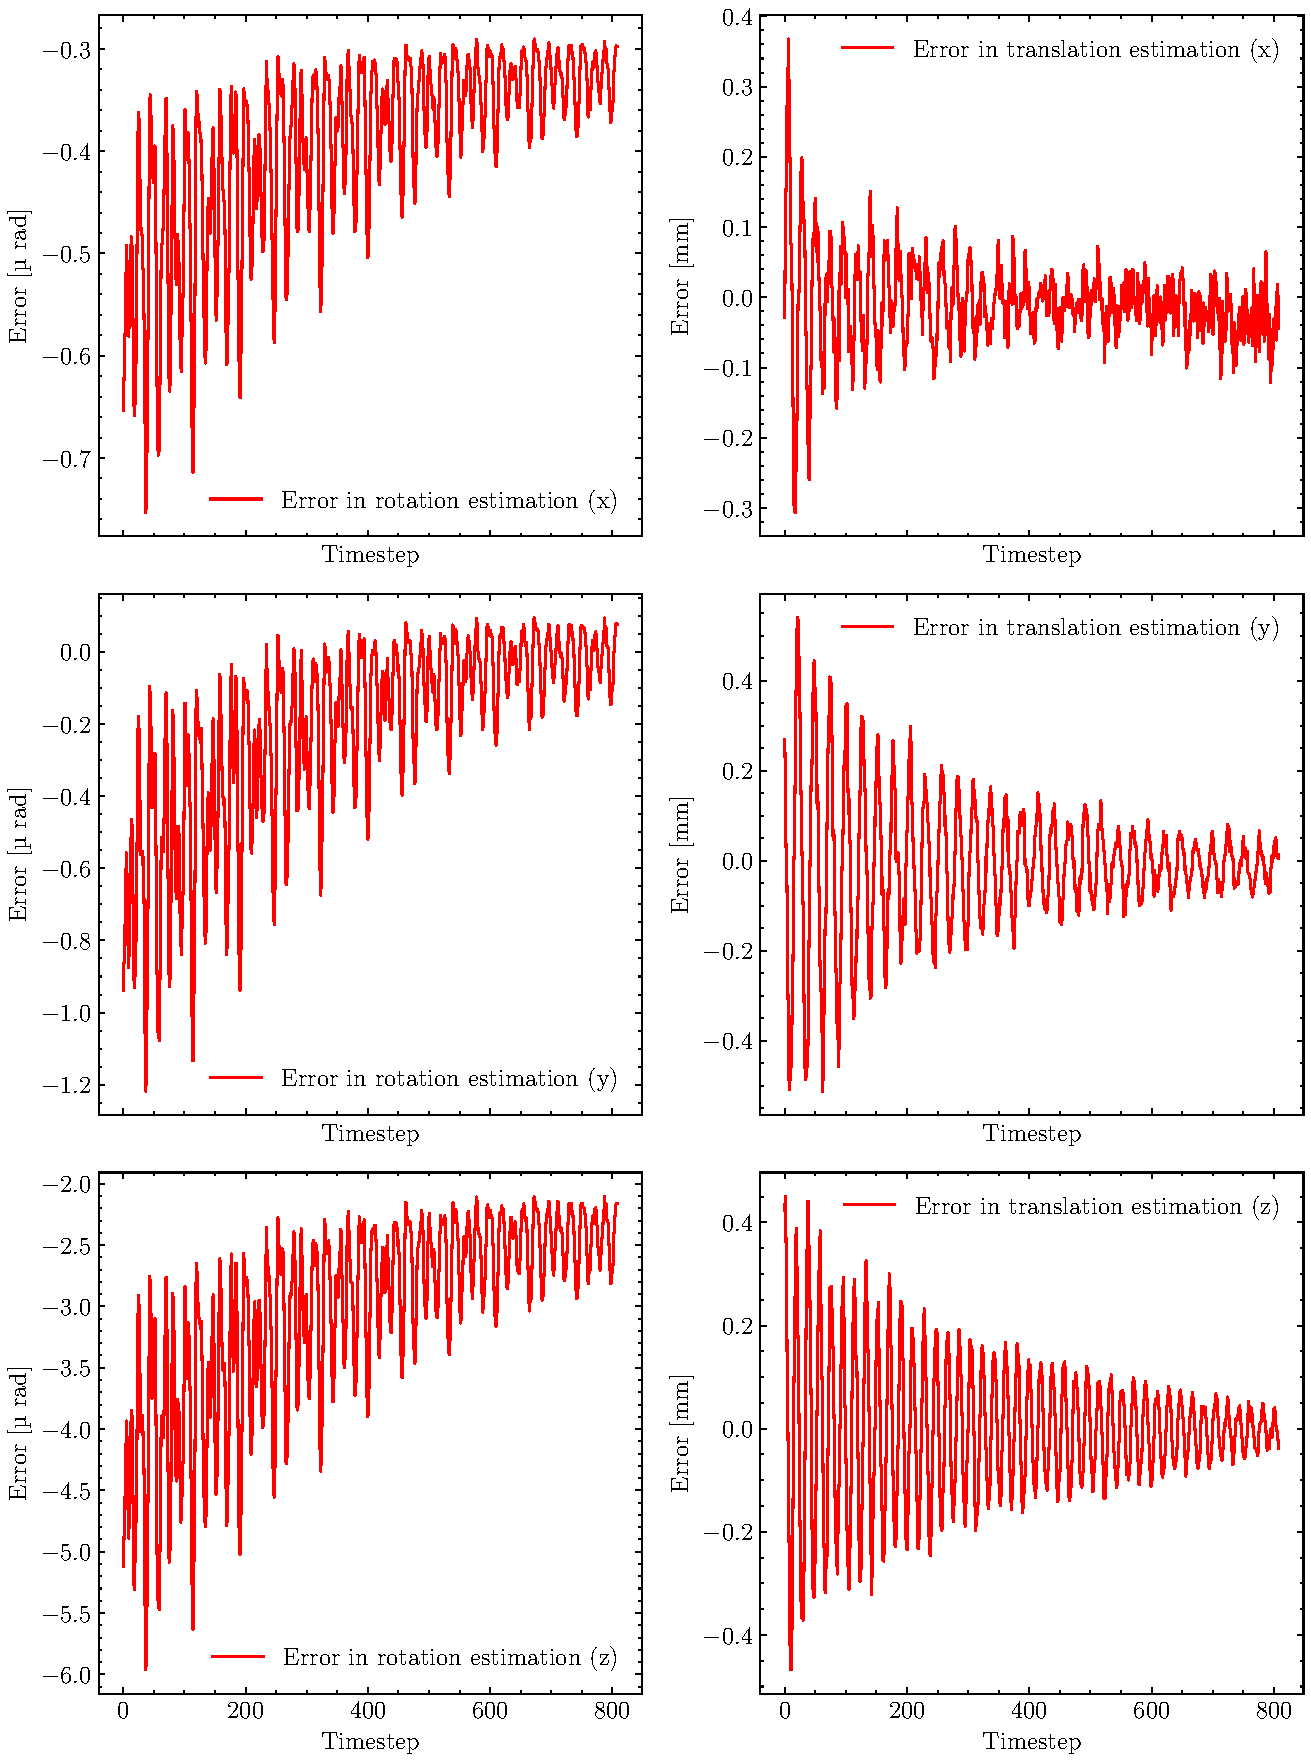
\includegraphics[scale=0.52]{images/fig_chapter4/nn_related/error_in_predicted_vs_ground_truth_resnet.pdf}
    \caption{Error in each DoF for ResNet}
    \label{fig:resnet_error}
\end{figure}


%% CNN-Transformer
\subsection{CNN-Transformer}
The network is structured in a way that the input goes through four \textbf{1D - Convolutional Layers} in sequence with \textbf{GELU} activation (non-linear). The output from these convolutional layers is fed to the \textit{Transformer Encoder}. Transformer Encoder has six layers with each layer having \textbf{Multi Headed Attention}, \textbf{Dropout}, \textbf{GELU} and \textbf{Layer Norm}. The output from the encoder layer goes into the output layers consisting of \textbf{Layer Normalization}, \textbf{Linear} layer, \textbf{GELU} non-linearity, \textbf{Dropout} and finally a \textbf{Fully Connected} layer to regress the output pose.

\begin{figure}[H]
    \centering
    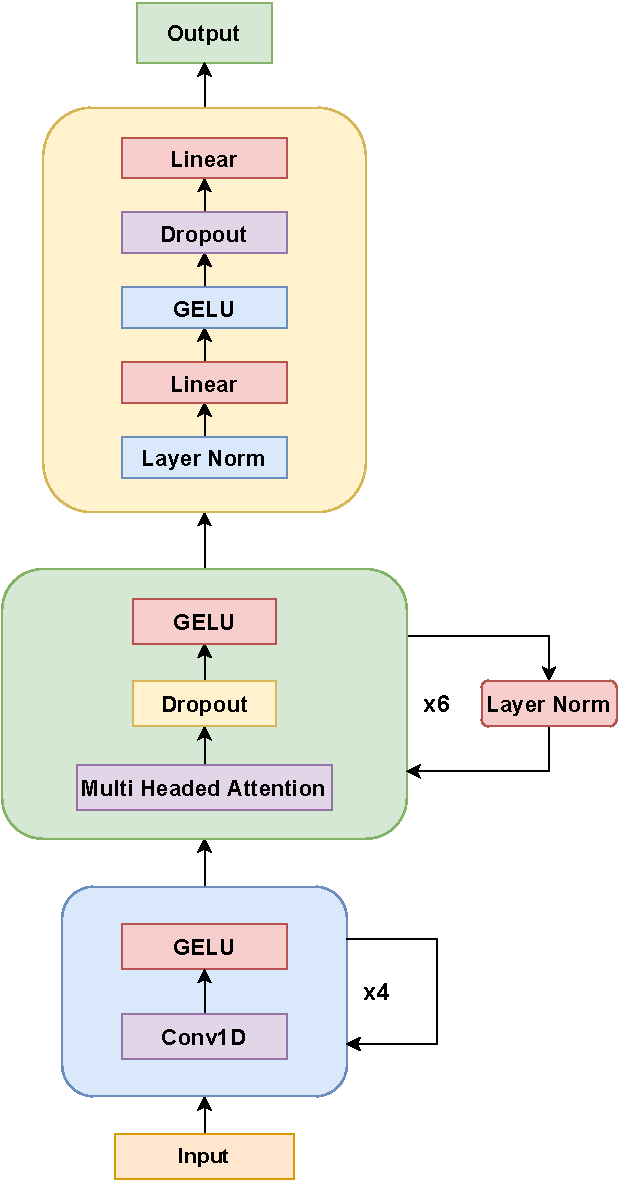
\includegraphics[scale=0.8]{images/fig_chapter2/nns/transformer_mt.pdf}
    \caption{CNN-Transformer Network Used}
    \label{fig:cnn_transformer_used}
\end{figure}

\subsubsection{Model Output Analysis}
Figure \ref{fig:cnn_trans_op_vs_gt} shows the model output vs ground truth plot for a 27 seconds video three linear DoF (x, y, z). The model can regress stabilization trajectory based on input IMU readings with very precision and the error is in a very low range of the order of micrometers ($ \mu m $) and micro radians ($ \mu \theta $).

\begin{figure}[H]
    \centering
    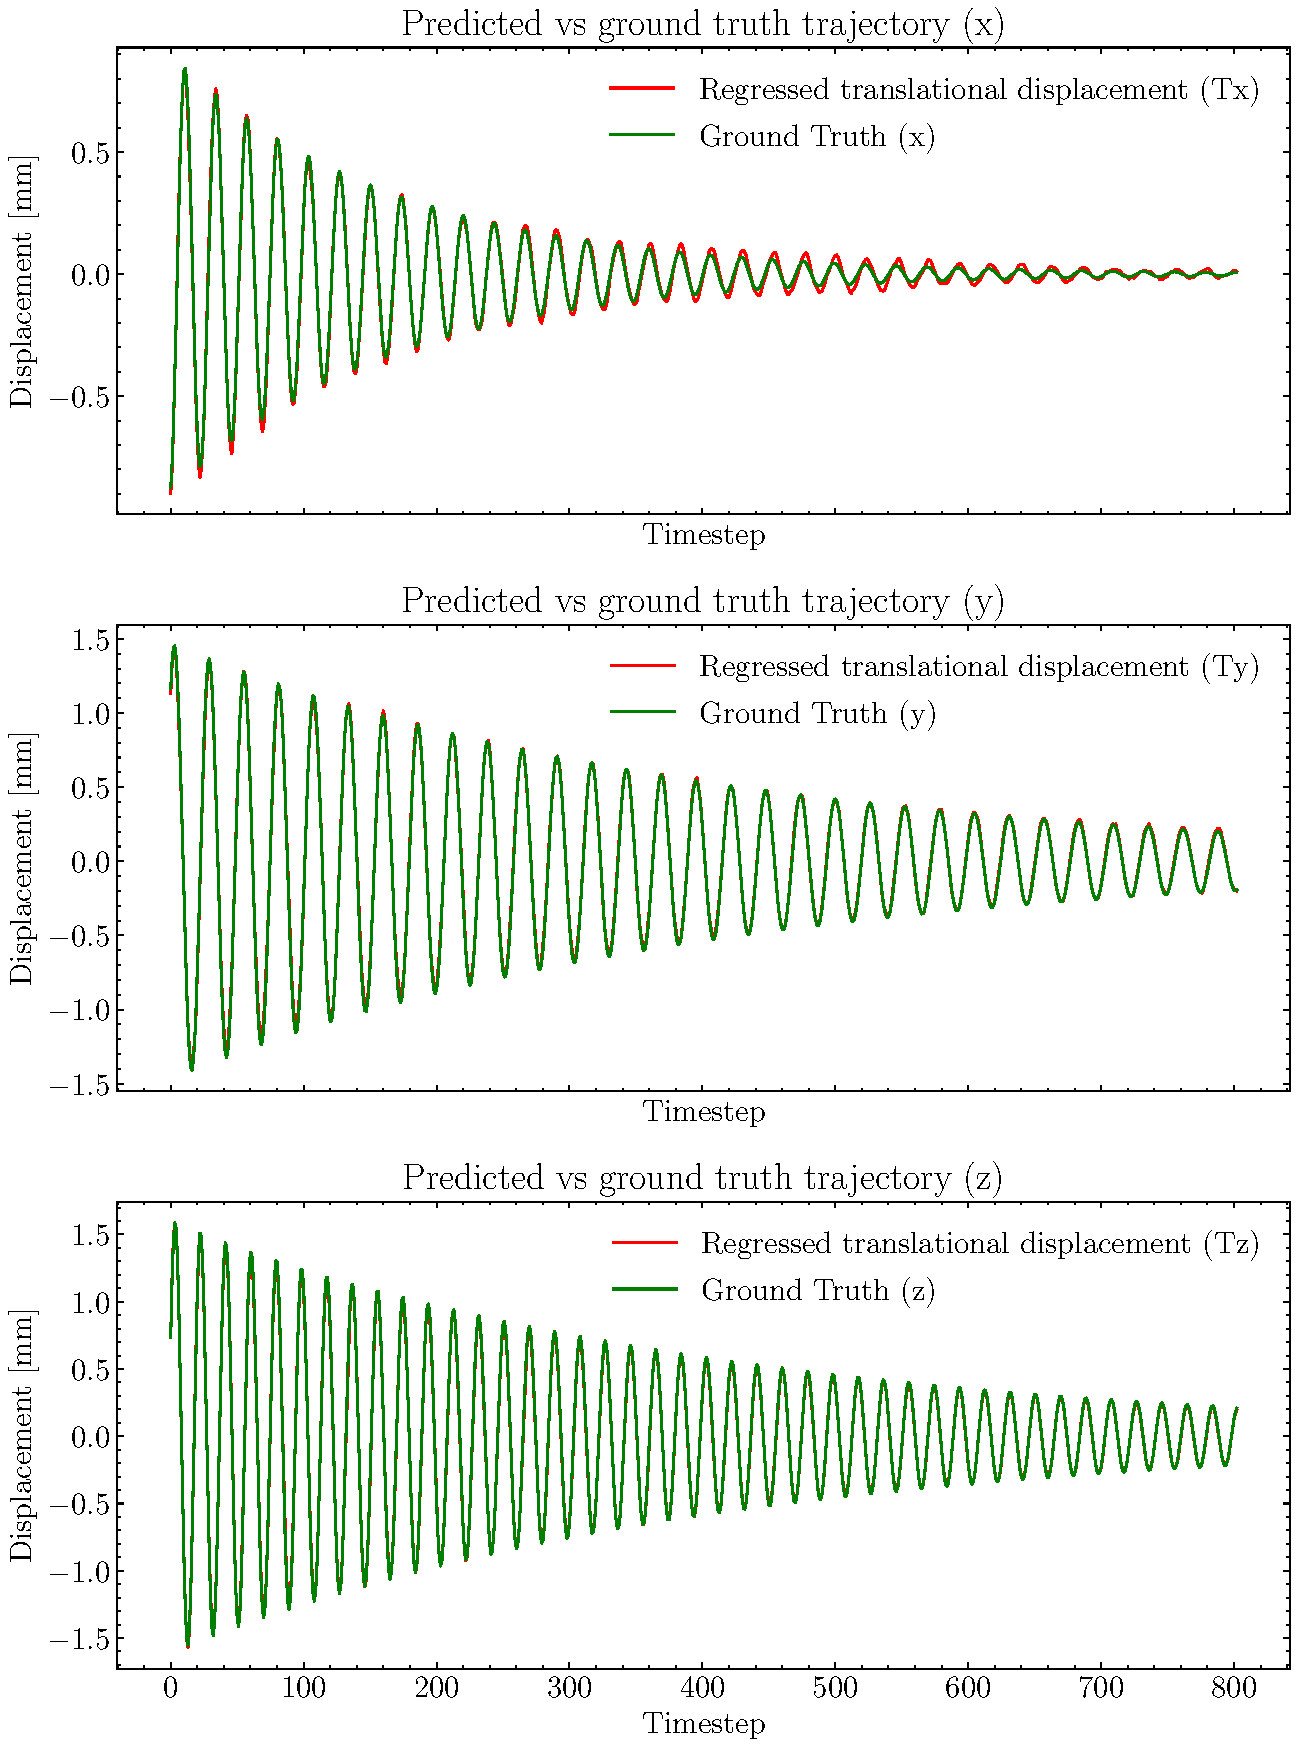
\includegraphics[scale=0.55]{images/fig_chapter4/nn_related/predicted_vs_ground_truth_transformer.pdf}
    \caption{Model prediction vs ground truth for CNN-Transformer}
    \label{fig:cnn_trans_op_vs_gt}
\end{figure}

\begin{figure}[H]
    \centering
    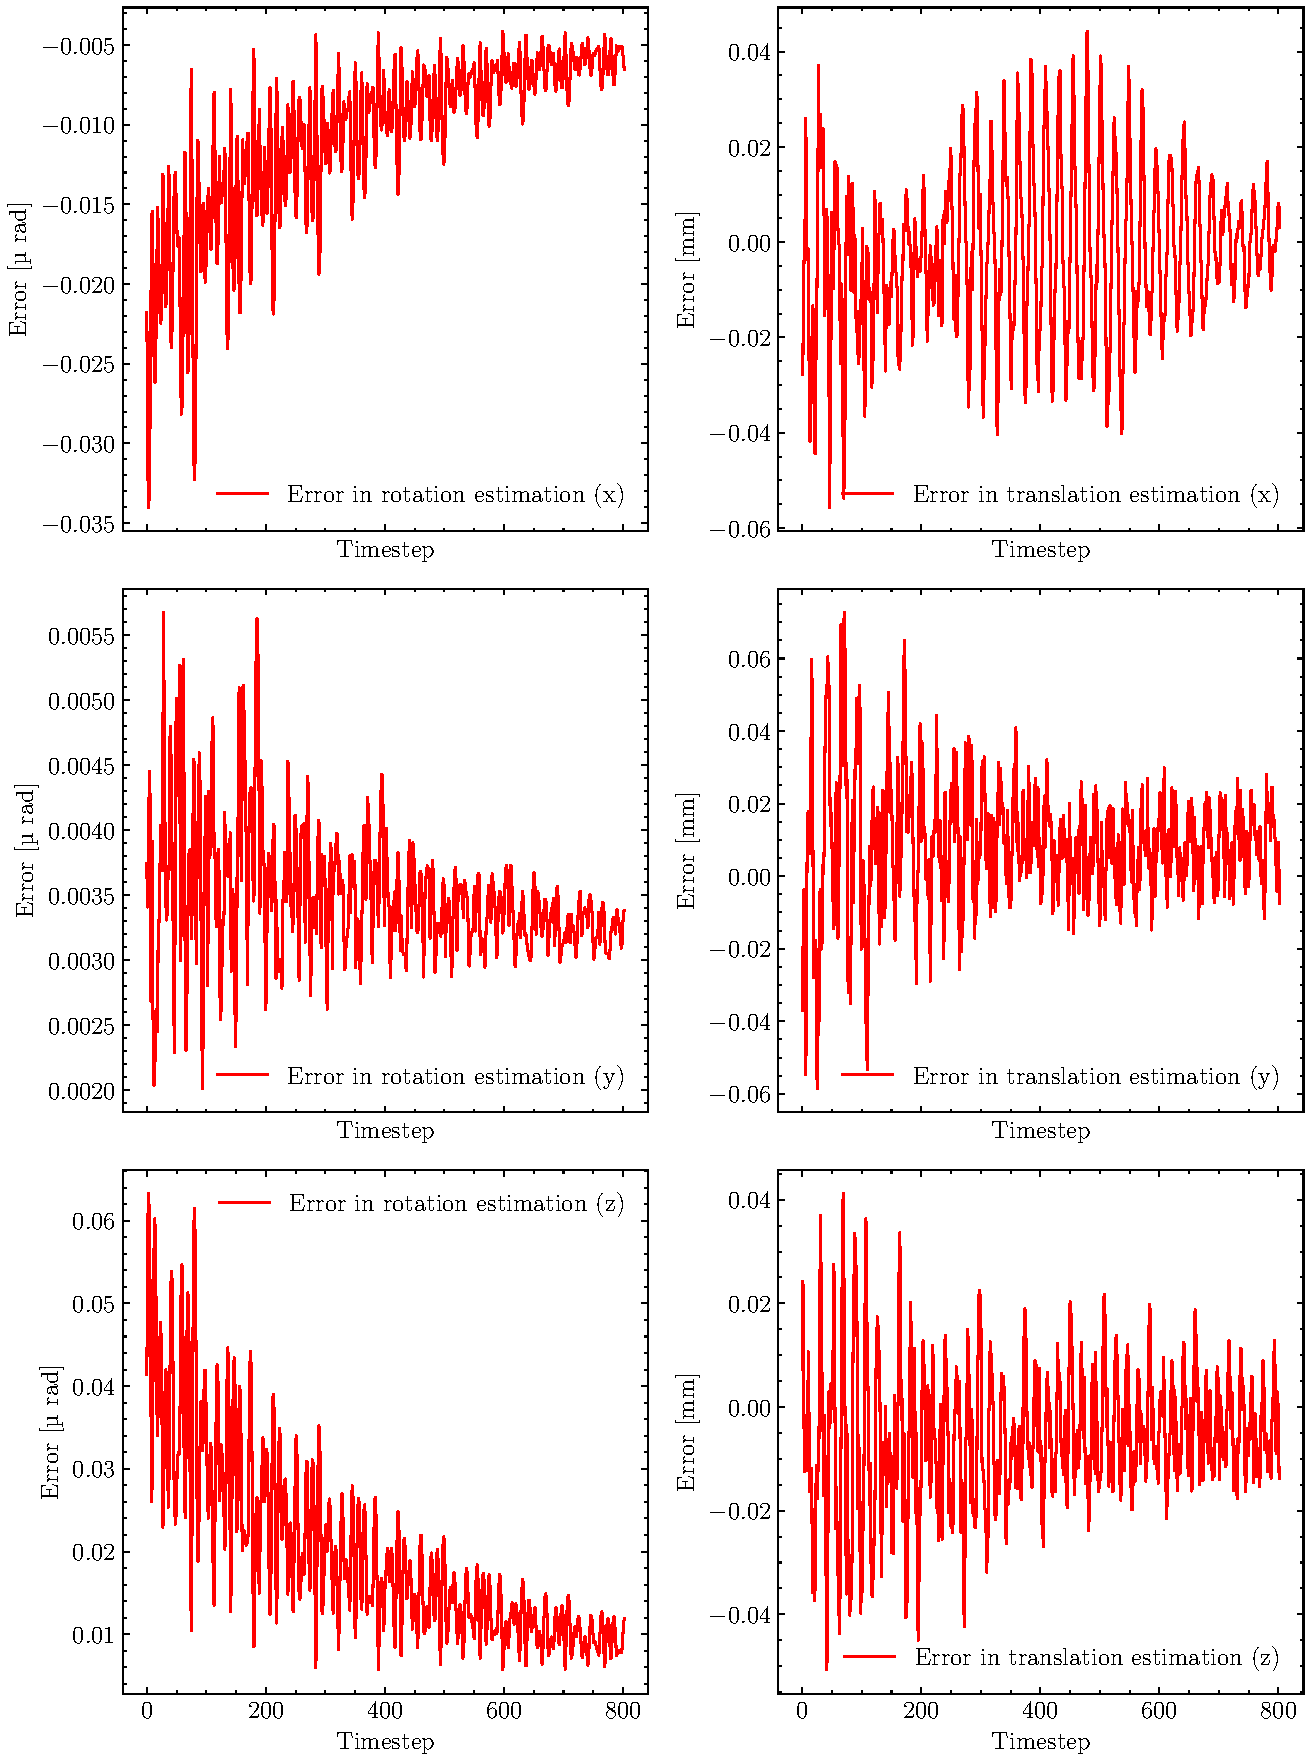
\includegraphics[scale=0.52]{images/fig_chapter4/nn_related/error_in_predicted_vs_ground_truth_transformer.pdf}
    \caption{Error in each DoF for CNN-Transformer predictions}
    \label{fig:cnn_trans_error}
\end{figure}

\subsection{Smoothing of Stabilization Trajectory}
The neural network is able to regress the stabilization trajectory accurately with the required precision. But the regressed trajectory is not smooth as show in figure \ref{fig:rough_mo_smooth_gt} and has sharp peaks and sudden changes. This is not acceptable as these rough peaks cause jitter in the stabilized video. To account for this, we implemented \textit{Trajectory-Smoothening} in our digital image stabilization pipeline as shown in figure \ref{fig:dis_smooth_pipeline}. An \textbf{Exponential Moving Average Filter} (Equation \ref{eqn:emaf}) is implemented to smooth the trajectory and minimise jitter. Figure \ref{fig:rough_mo_smooth_mo} shows the effect of this filter on the model output.

\begin{figure}[H]
    \centering
    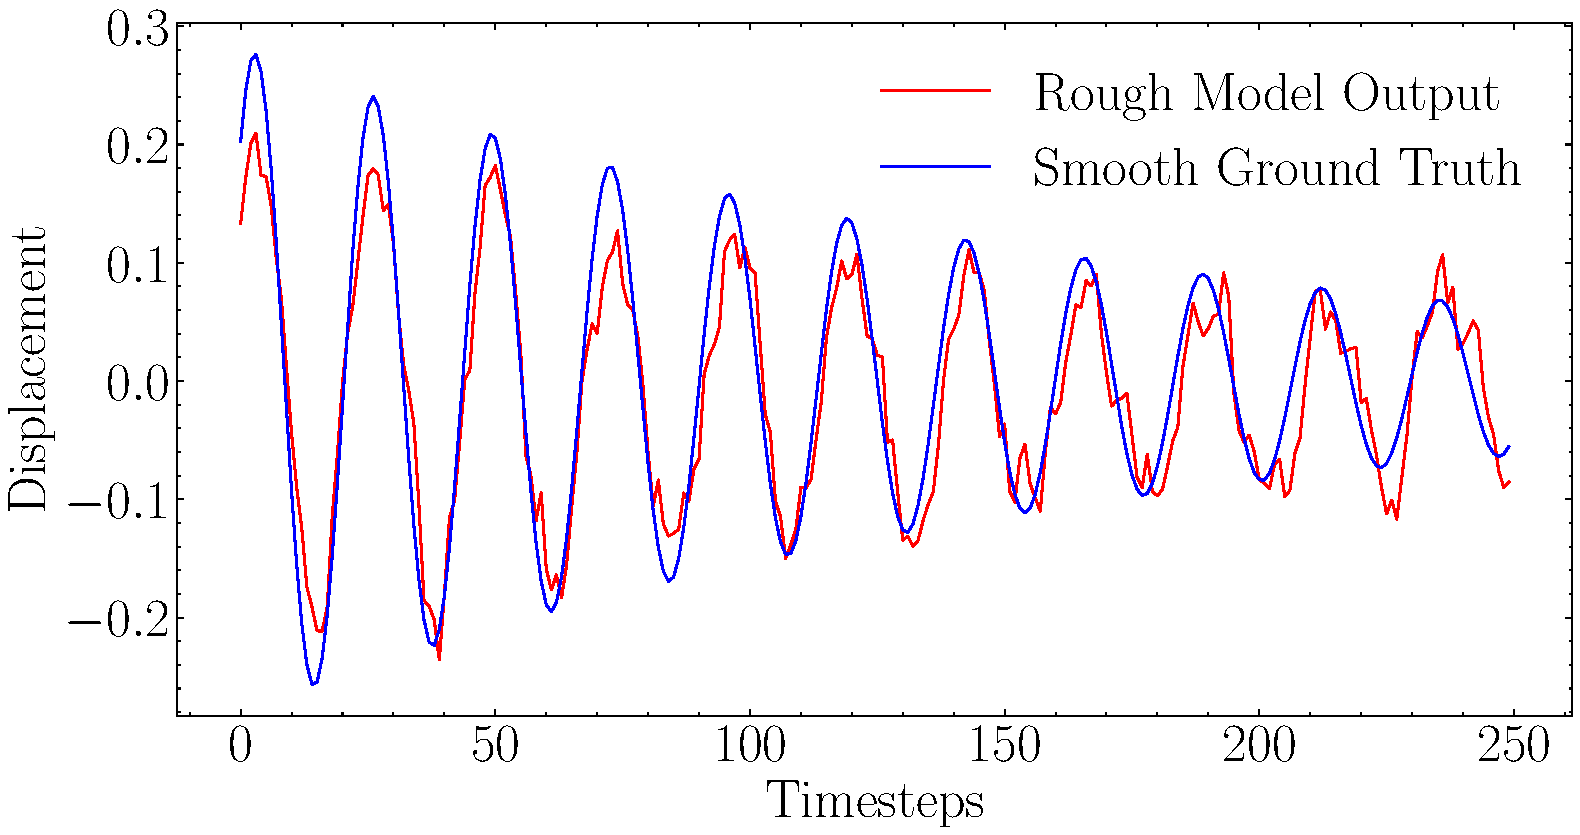
\includegraphics[scale=0.41]{images/fig_chapter4/nn_related/rough_mo_smooth_gt.pdf}
    \caption{Rough regressed vs smooth ground-truth trajectory}
    \label{fig:rough_mo_smooth_gt}
\end{figure}

\begin{equation}
    y_t = x_t  \frac{S}{1+H_l} + y_{t-1}(1 - \frac{S}{1+H_l})
    \label{eqn:emaf}
\end{equation}

Where $ y_t $ is the smoothed signal and $ y_{t-1} $ is the smoothed signal at previous time-step. $ x_t $ is the signal value at current time-step. $ S $ is the smoothing factor and $ H $ is the horizon length. We need to be careful with smoothing the stabilization trajectory because the more we smooth the higher will be the error introduced in the stabilization trajectory.


\begin{figure}[H]
    \centering
    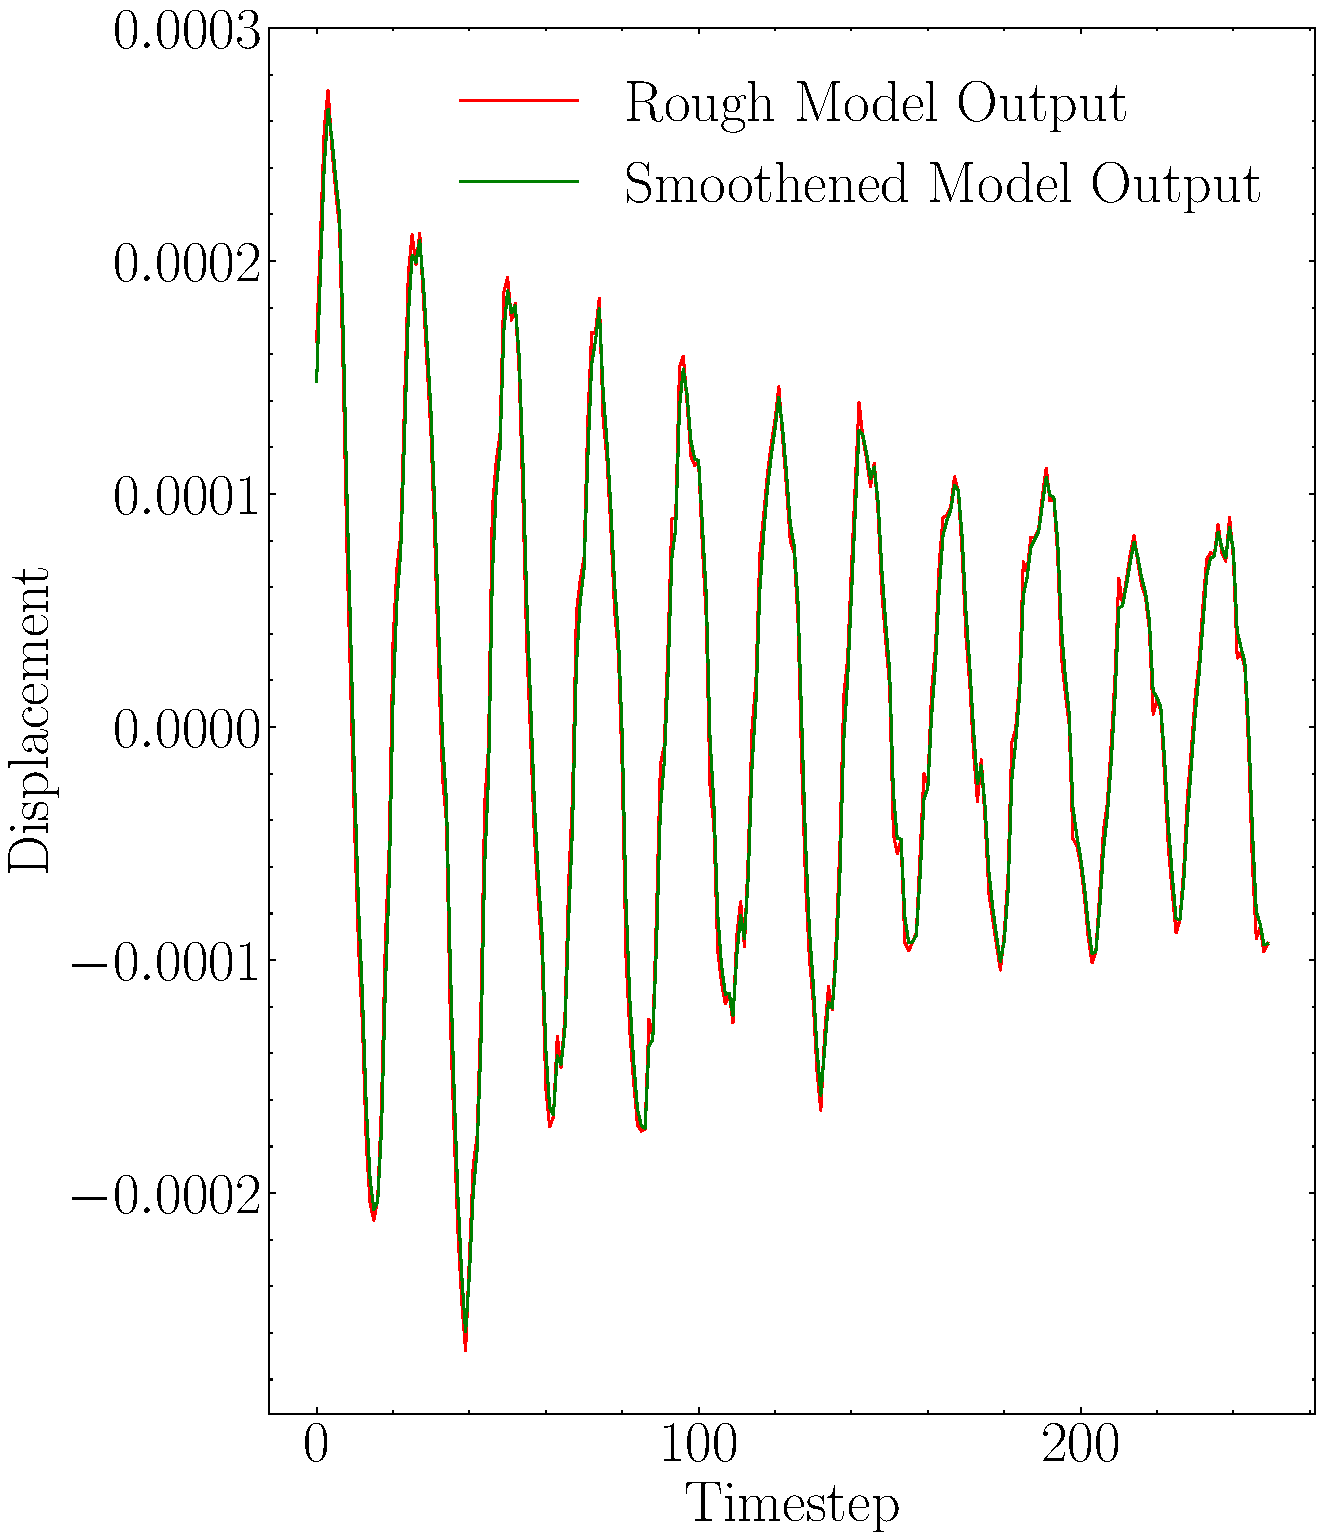
\includegraphics[scale=0.25]{images/fig_chapter4/nn_related/rough_mo_smooth_mo.pdf}
    \caption{Smoothed model output vs raw model output}
    \label{fig:rough_mo_smooth_mo}
\end{figure}

\begin{figure}[H]
    \centering
    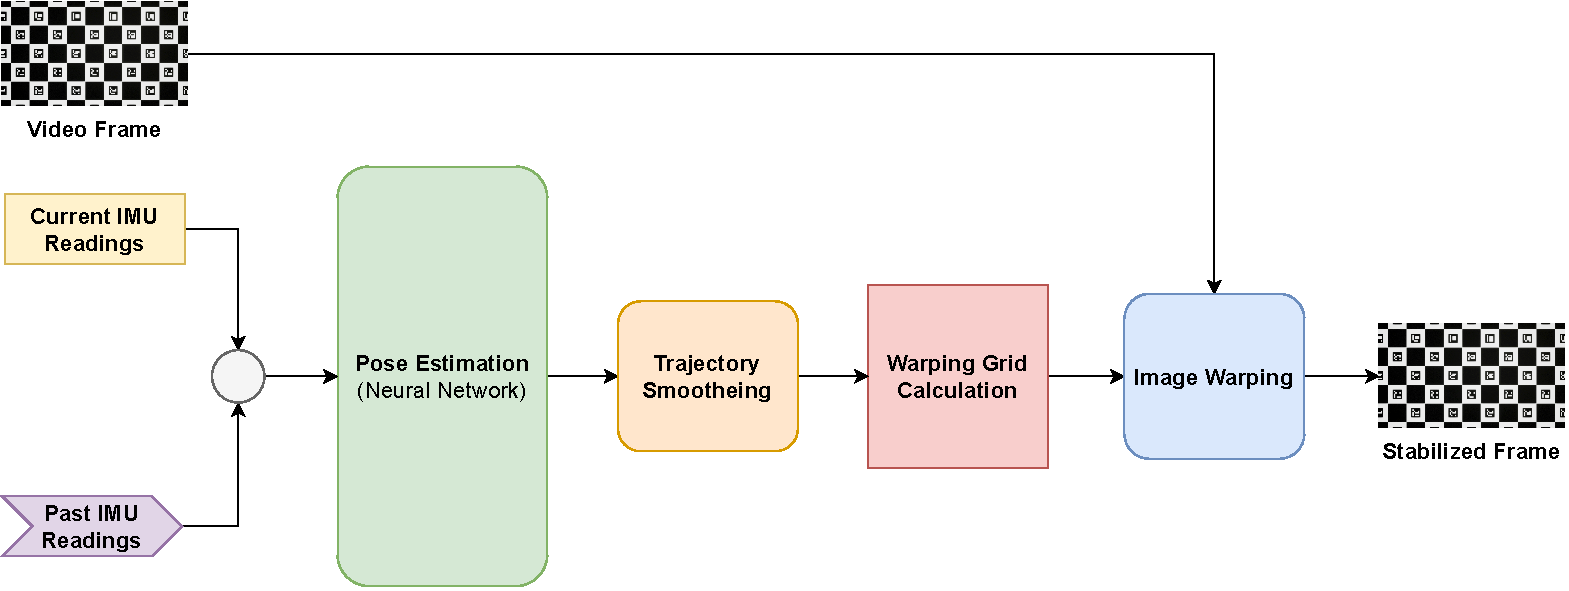
\includegraphics[scale=0.78]{images/fig_chapter4/dis_smooth_pipeline.pdf}
    \caption{DIS pipeline with trajectory smoothing}
    \label{fig:dis_smooth_pipeline}
\end{figure}




%% ############################## Mathematics ########################################

% \section{Warping Grid Estimation}
% In our \textit{Digital Image Stabilization Pipeline} (figure \ref{fig:dis_pipeline}) after getting the relative pose from stabilization trajectory, we need to estimate the warping grid. This warping grid is applied to the image coming from the camera with a crop-ratio of 95 percent (5 percent of the image area will be cropped). These series of warped images based on the pose estimated results into the output stabilized video. 

% For warping grid calculation we need to estimate \textit{homography} between stabilized trajectory frame (no actual frame in our case because our prediction is always relative to the stabilized trajectory itself) and the current frame. We assume two image points \textbf{\textit{x}} at times $ t_{i} $ (equation \ref{eqn:x_ti}) and $ t_{j} $ (equation \ref{eqn:x_tj}) from scene points \textbf{X} as shown in figure \ref{fig:dis_point_scene}.

% \begin{figure}[H]
%     \centering
%     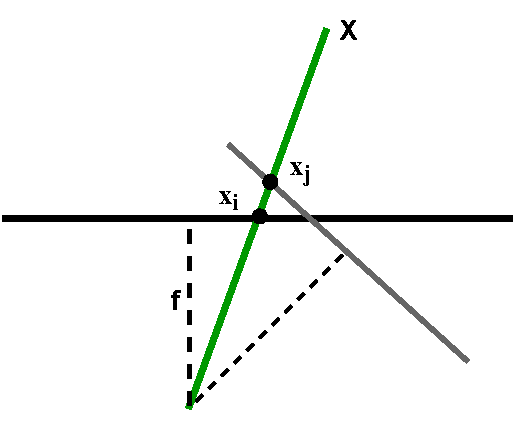
\includegraphics[scale=0.8]{images/fig_chapter4/dis_point_scene.pdf}
%     \caption{Scene points at different time-steps}
%     \label{fig:dis_point_scene}
% \end{figure}

% \begin{equation}
%     \lambda_{i} x_{i} = K(R(t_i)X + p(t_i))
% \label{eqn:x_ti}
% \end{equation}

% \begin{equation}
%     \lambda_{i} x_{j} = K(R(t_j)X + p(t_j))
% \label{eqn:x_tj}
% \end{equation}

% Where, $ R $ is the camera rotation, $ p $ is the camera position and $ K $ is the camera projection matrix (3D to 2D). In our case we have both translation and rotation (although very small). To warp, we need to transform points from camera i to camera j.

% \begin{equation}
%     \lambda_{i} x_{j} = KR(t_j)R(t_i)^{T} \lambda_{i} K^{-1} x_{i} - K(R(t_j)R(t_i)^{T} p(t_i) + p(t_j))
% \label{eqn:homography}
% \end{equation}

% \begin{equation}
%     \lambda_{i} x_{j} = K(R_{rel} \lambda_{i} K^{-1} x_i + p_{rel})
% \label{eqn:homography_simplified}
% \end{equation}

% The relative rotations and translations between two frames (i and j) are estimated using equations \ref{eqn:rel_r} and \ref{eqn:rel_t}. These are the values ($ R_{ij} $ and $ t_{ij} $) neural networks were trained to predict. 

% \begin{equation}
% R_{ij} = R_i R_i^T
% \label{eqn:rel_r}    
% \end{equation}

% \begin{equation}
% t_{ij} = t_i - R_{ij}t_j
% \label{eqn:rel_t}
% \end{equation}

%% ############################## Mathematics ########################################




\section{Model Deployment}
Figure \ref{fig:dis_smooth_pipeline} shows the digital image stabilization pipeline and our goal is to minimise the time taken at each step. The video (images) are coming at 60 FPS from the camera that has 4K resolution (3840x2160 pixels). We ideally have 1/60 seconds (16.67 ms) to complete all the steps of the DIS pipeline. In this pipeline, model inference and stabilization grid calculation take most of the given time. Stabilization grid calculation is a series of matrix multiplications and has been already optimized. Thus, low inference latency is highly desirable.

\subsection{Making Models Fast}
There are many techniques to reduce the inference latency of neural network models. Using these methods may reduce the performance of a neural network but are essential for deployment as models in their original form may not be usable at all. Some of the popular methods are discussed below.

\subsubsection{Quantization}
This is a very common approach used to to tackle high latency of deep learning models especially in case of edge hardware deployment. We can \textbf{quantize} the model by by converting the weights from floating point (32-bits) to integers (8 bits). This decreases the memory requirements significantly while also improving CPU and hardware accelerator latency \citep{FastModels}. 

Another recent approach is to convert the model to \textbf{half-precision} (16-bit floating point). It acts as a middle ground between FP32 and INT8 and the performance trade-off is reduced while decreasing the model size. Another very important thing to note is that not all layers have high latency and thus selective weight quantization for layers like convolution layers can also be done making the performance trade-off even smaller.

\subsubsection{Making Models Lean}
The field of deep-learning is growing at a fast pace and we have a large selection of various neural network architectures some even with more than 100 Billion trainable parameters. But while developing deep-learning models, our goal should be to use models with the lowest number of parameters and complex layers while keeping the performance acceptable.

\subsection{Model Inference Latency on various Hardware}
Various trained models (CNN, ResNet and Transformer) are checked for inference latency and the results are summarised in table \ref{tab:model_inference}. Models were also quantized or converted to ONNX for deployment. The models were inferred 1000 times and the result in the table is an average.

% Sim Vibration characteristics
 \begin{table}[H]
\centering
\begin{tabular}{ l | L | L | L }
    
    Architecture  & 
    Format & 
    No. of Parameters &
    Inference Latency (ms) \\
    \hline
    
    CNN & 
    PyTorch Checkpoint (.ckpt)  & 
    745,375  &
    -  \\
    
    
    CNN & 
    ONNX (.onnx)  & 
    745,375   &
    -  \\
    
    ResNet & 
    PyTorch Checkpoint (.ckpt)  & 
    1.85 Million &
    -  \\
    
    
    ResNet & 
    ONNX (.onnx)  & 
    1.85 million  &
    -  \\
    
    CNN-Transformer & 
    PyTorch Checkpoint (.ckpt)  & 
    225,356  &
    -  \\
    
    
    CNN-Transformer & 
    ONNX (.onnx)  & 
    225,356  &
    -  \\

    \hline
   
\end{tabular}
    \caption{Inference latency of different models}
    \label{tab:model_inference}
\end{table} %%%%


This chapter contained all the steps we took and the techniques we used to successfully realise digital image stabilization without incorporating any image observations into the algorithm but rather fully relying on inertial measurement data. Various neural network architectures for pose estimation were examined. Throughout the experiments transformer networks outperformed standard CNN architectures for this task. The importance of post-processing the neural network output with a moving average filter to smooth out the jitter was also discussed. In the end a run-time analysis of each architecture was performed that showed that the latency  requirements were met.


